% +------------------------------------+
% |   Generated by www.docx2latex.com  |
% |   Version: 2.0.0                   |
% +------------------------------------+

\documentclass[11pt]{book}

\usepackage{adjustbox}
\usepackage{caption}
\usepackage{float}
\usepackage[T1]{fontenc}
\usepackage{graphicx}
\usepackage{hhline}
\usepackage[utf8]{inputenc}
\usepackage{multicol}
\usepackage{multirow}
\usepackage{subcaption}
\usepackage[normalem]{ulem}
\usepackage[svgnames]{xcolor}
\usepackage[paperheight=29.69cm,paperwidth=21.01cm,left=2.54cm,right=2.54cm,top=2.54cm,bottom=2.54cm]{geometry}
\usepackage[hidelinks]{hyperref}


\setlength\parindent{0pt}
\renewcommand{\arraystretch}{1.3}


\title{6 Dev Round 3 -Automatic Clamp Placement}

\begin{document}
\maketitle

\vspace{1\baselineskip}
\subsection{Goal}

The goal of the third round is to address the issues observed in the previous round and to test the rest of the automatic process that were not included in the previous round \textit{\textcolor[HTML]{B7B7B7}{(see \uline{4.1.4 DiRT Clamping Assembly Process Task List (v1)})}}. This was expected to be challenging due to inaccuracy. The following list shows an overview of the technical development in this round to achieve the goal. 

\begin{itemize}
	\item \textbf{Mechatronics}

\begin{itemize}
	\item Implemented docking adapter

	\item Addressed issues found in clamp electronics

\end{itemize}
	\item \textbf{Controller / Firmware}

\begin{itemize}
	\item Added stall protection in motion control

	\item Process Execution Controller switched from GH interface to standalone GUI application

\end{itemize}
	\item \textbf{CAD Design Software}

\begin{itemize}
	\item Design software switched to Rhino Python

\end{itemize}
	\item \textbf{Task and Motion Planning }(TAMP)

\begin{itemize}
	\item Developed Flowchart Formulation method for task planning

	\item Established high-level and low-level tasks and planning template

	\item Developed planning method to handle Taught configuration

	\item Developed Non-Sequential Multimodal Motion Planning (MMMP) solver

	\item Developed Kinematic Robotic Tool Models

	\item Integrated Post-planning Trajectory Smoothing

\end{itemize}
\end{itemize}
Majority of the development effort was expanded to develop the software infrastructure that would allow automatic task and motion planning (TAMP). Many of the related developments and discoveries presented in this chapter were created in collaboration with YiJiang Huang (from MIT Architecture) who specialises in TAMP for Construction Tasks. The level of software automation would not have been possible without this collaboration.

No new demonstrator structure was created for this round. The timber beams of the BusStop Pavilion were used again for testing and demonstration. 

\subsubsection{DiRT Clamping Assembly Process Task List (v2)}

The robotic process task list is a revision from Section \uline{4.1.4 DiRT Clamping Assembly Process Task List (v1)} after incorporating the lessons learned from \uline{5.5.3 Narrow Passage Problem}. Approach and Retract targets are added to the beginning or the end of Free Motions to circumvent the Narrow Passage problems. However, this added many small motions to the overall task list.

In order to maintain a high level overview of the process, I developed a task group concept that is able to represent a group of tasks in an abstract way. This is referred to as \textbf{High-Level Tasks}. For example, it can contain a free motion to go to a target, linear motions between approach and retract points, and tool operations such as gripper movements and clamp movements. 

The following table lists out the High-Level Tasks. The Lower-Level Tasks for each High-Level Tasks are listed in \uline{6.3.5.2 Expansion to Low-Level Tasks}. 

\begin{table}[H]
\begin{adjustbox}{max width=\textwidth}
\begin{tabular}{p{11.36cm}p{4.51cm}}
\hline
\multicolumn{1}{|p{11.36cm}}{{\footnotesize \textbf{Task Description}}} & 
\multicolumn{1}{|p{4.51cm}|}{{\footnotesize \textbf{Shortened Name}}} \\ 
\hline
\multicolumn{2}{|p{15.87cm}|}{\begin{enumerate}
	\item {\footnotesize \uline{Place all necessary clamps onto the PA structure (repeat for all clamps)}}} \\ 
\hline
\multicolumn{1}{|p{11.36cm}}{{\footnotesize Robot picks up a clamp from where the clamps are stored.}} & 
\multicolumn{1}{|p{4.51cm}|}{{\footnotesize PickClampFromStorage}} \\ 
\hline
\multicolumn{1}{|p{11.36cm}}{{\footnotesize Robot places the clamp onto the PA structure and releases it.}} & 
\multicolumn{1}{|p{4.51cm}|}{{\footnotesize PlaceClampToStructure}} \\ 
\hline
\multicolumn{2}{|p{15.87cm}|}{	\item {\footnotesize \uline{Bring the next beam to be assembled}}} \\ 
\hline
\multicolumn{1}{|p{11.36cm}}{{\footnotesize Robot picks up a gripper from where the gripper is stored.}} & 
\multicolumn{1}{|p{4.51cm}|}{{\footnotesize PickGripperFromStorage}} \\ 
\hline
\multicolumn{1}{|p{11.36cm}}{{\footnotesize Robot picks up the next beam from the operator at the loading station}} & 
\multicolumn{1}{|p{4.51cm}|}{{\footnotesize PickBeamFromStorage}} \\ 
\hline
\multicolumn{2}{|p{15.87cm}|}{\begin{enumerate}
	\item {\footnotesize \uline{If this is a beam with no clamps}}} \\ 
\hline
\multicolumn{1}{|p{11.36cm}}{{\footnotesize Robot places the beam on the ground. The operator fixes it.}} & 
\multicolumn{1}{|p{4.51cm}|}{{\footnotesize PlaceBeamInClamp}} \\ 
\hline
\multicolumn{2}{|p{15.87cm}|}{	\item {\footnotesize \uline{If this beam used clamps}}\end{enumerate}
} \\ 
\hline
\multicolumn{1}{|p{11.36cm}}{{\footnotesize Robots and clamps move in synchronisation to clamp the joints.}} & 
\multicolumn{1}{|p{4.51cm}|}{{\footnotesize AssembleBeamWithClamps}} \\ 
\hline
\multicolumn{1}{|p{11.36cm}}{{\footnotesize Robot places the gripper back to its storage location.}} & 
\multicolumn{1}{|p{4.51cm}|}{{\footnotesize PlaceGripperToStorage}} \\ 
\hline
\multicolumn{2}{|p{15.87cm}|}{\end{enumerate}
	\item {\footnotesize \uline{Retrieve all clamps from the PA structure (repeat for all clamps)}}} \\ 
\hline
\multicolumn{1}{|p{11.36cm}}{{\footnotesize Robot picks up a used clamp from the PA structure.}} & 
\multicolumn{1}{|p{4.51cm}|}{{\footnotesize PickClampFromStructure}} \\ 
\hline
\multicolumn{1}{|p{11.36cm}}{{\footnotesize Robot places the clamp back in its storage location.}} & 
\multicolumn{1}{|p{4.51cm}|}{{\footnotesize PlaceClampToStorage}} \\ 
\hline
\end{tabular}
\end{adjustbox}
\end{table}
\vspace{1\baselineskip}
\subsection{Literature Review}

\subsubsection{Workflow for Generating Assembly Programmes}

In this thesis, the generation of robotic assembly programmes is hypothesised to be similar to the generation of machining processes. Both of them require the creation of robotic trajectories (analogous to toolpaths) while satisfying a list of machine constraints (e.g. avoiding collisions). Therefore, the development in this thesis follows a similar workflow to that of CAM software for machining for testing this hypothesis.

Existing CAM software for machining follows a structured workflow that typically begins with importing a CAD model containing the geometry of the part to be machined. A CNC programmer (also known as machinist, engineer, technician) then defines the CNC machine’s kinematics, stock material setup, fixture geometry (collision geometry) and tools. The CAM software then analyses the geometry and generates a series of toolpaths for each operation while considering the machine's constraints, such as spindle speed, feed rate, and tool engagement. After generating the toolpaths, the programmer reviews the simulation results and makes adjustments if needed. Once the tool paths are satisfactory, the CAM software creates G-code instructions, which are sent to the CNC machine for execution.

In comparison, the workflow for generating robotic assembly programmes can also start with the Assembly Model \textit{\textcolor[HTML]{B7B7B7}{(see \uline{5.3.13 Assembly Model Data Structure and Functions})}} containing the geometry and design information of the timber structure. A production engineer\footnote{ The title of this persona is has no precedence. I name it the ‘Production Engineer’ to avoid confusion with existing ‘construction planner’ that plans construction site or ‘programmer’ that writes software.} then defines the setup of the robotic environment, and makes decisions about which tools to use and what assembly strategy to use. A software then generates the assembly programme, considering factors such as assembly sequence, robot kinematics, joint assembly tools and collisions. Similar to CAM machining workflows, the generated programme is reviewed and adjusted as needed before being sent to the robotic system for execution.

Despite the similarities between generating robotic assembly programmes and CAM machining programmes, there are notable differences. Assembly operations focus on the manipulation and joining of components rather than material removal in machining. Additionally, robotic assembly processes have more complex constraints \href{https://www.zotero.org/google-docs/?DQYwa5}{(Wang et al., 2021)}. While CAM software for machining has reached a high level of automation and optimization, software for generating robotic assembly programmes has not yet achieved the same maturity, partly due to the recent adoption of robotics for spatial construction tasks. Challenges in generating robotic assembly programmes include accurately modelling and simulating the assembly process, accounting for factors like assembly tools, joint connections, and structural stability. Furthermore, the software must generate efficient and feasible assembly sequences, considering accessibility, reachability, and potential collisions.

This thesis aims to address these challenges by developing and testing workflows that are inspired by CAM machining. The goal is to create an efficient fabrication-aware design process that extends to the robotic assembly constraints. By adopting the patterns established for CAM machining workflows, the development process can avoid reinventing the wheel while addressing the unique challenges of robotic assembly in timber construction.

\vspace{2\baselineskip}
\subsubsection{Multimodal Motion Planning (MMMP)}

In the previous round, motion planning was introduced as finding the path between two targets. However, the many more chained robotic motions in this round \textit{\textcolor[HTML]{B7B7B7}{(see \uline{6.2.2 DiRT Clamping Assembly Process Task List (v2)}) }}will require substantially more effort to chain the robotic configuration correctly between MP. In addition, the manually performed backtracking in the last round would have to be automated to handle this many more chained motions \textit{\textcolor[HTML]{B7B7B7}{(see \uline{5.3.14.2 Motion Planning})}}. 

Multimodal Motion Planning (MMMP) is an advanced approach to robotic motion planning that takes into consideration different kinematic configurations, different motion constraints and different types of actuators \href{https://www.zotero.org/google-docs/?a7FuIN}{(Hauser $\&$ Latombe, 2010; Hauser $\&$ Ng-Thow-Hing, 2011)}. MMMP expands the capabilities of single-query motion planning algorithms \textit{\textcolor[HTML]{B7B7B7}{(see \uline{5.2.7.5 Selecting Motion Planning Algorithms})}} to perform more complex tasks.

MMMP addresses these limitations by incorporating the concept of multiple modes into the planning process, enabling the robot to switch between different operational modes as needed to achieve the desired task more efficiently. The mode definition relevant to the DiRT Assembly Process includes the following components:

\begin{itemize}
	\item \textbf{Kinematic chain configuration }- The attached objects after the kinematic chain of the robot, such as docking adapter, clamps, grippers and beams.

	\item \textbf{Kinematic tool geometry} - Position of the clamp jaw and gripper fingers depending on whether they are open or close.

	\item \textbf{ACM }- Objects that are allowed to collide when they perform a certain part of the operation, such as joint closure.

	\item \textbf{Motion Type} - Linear vs Free motion

\end{itemize}
The mode definition allows the planner to understand the difference between different planning requirements in different parts of the operation. The MMMP solver used in this thesis was developed in collaboration with YiJiang Huang. The solver is described in the later development sections \textit{\textcolor[HTML]{B7B7B7}{(see \uline{6.3.5.7 Multimodal Motion Planning (MMMP) Solver} and \uline{6.3.7 Non-Sequential Planning Order})}} and in YiJiang’s PhD dissertation \href{https://www.zotero.org/google-docs/?R37lZz}{(Huang, 2022)}.

\subsubsection{Robot Targets - Taught Configuration and Cartesian Pose}

In order to specify the motion of a robotic arm, a program must be created. This is often achieved by a symbolic programme, written in a manufacturer-specific language such as Rapid for ABB robots and KRL for Kuka robots. The programme would contain a number of targets which the robot can pass through or stop at. These targets can be specified as \textbf{Robot Configurations}, a list of position values corresponding to each robot joint, or \textbf{Cartesian Poses}, a 6 DOF position and orientation definition.

For industrial automation with repetitive targets, the targets are typically specified by configurations. These would be created by the production engineer or programmer using a joystick to jog the arm to the intended target and record the joint values at that moment. This process is referred to as ‘teaching’. Teaching has to be performed in the production environment using the real robot, with tools and workpieces attached to the robot to accommodate deflection due to payload. The recorded configurations are known as \textbf{Taught Configurations}. If accurate alignment is needed, the jogging can be performed in small increments until good alignment is confirmed. This has to be repeated for every key position where alignment is important. 

Industrial robotic arms typically have good repeatability, meaning it is capable to go back to this taught target under the same payload. For performing repetitive tasks, this is largely sufficient. However, it is important to note that repeatability is different from ‘accuracy’, which is a measurement of its ability to reach an uncalibrated target. 

In cases where the target is not in a fixed position (e.g. position of an object located by a camera), or if the targets cannot be calibrated one by one, it is useful to specify them using a Cartesian Pose. This pose is often extracted from a digital model that estimates where the targets should be in relation to the robot base. The configuration of the robot joints must therefore be calculated using inverse kinematics (IK) calculation. 

However, the accuracy of IK calculation depends on the accuracy of the robot kinematics model, payload and the choice of configuration used to reach the pose. For example, high-DOF robots can have many different IK solutions, and a more stretched configuration can result in more defection. 

\subsection{Development}

\subsubsection{Ground Platform Redesign}

In order to reduce the planning difficulty caused by the side-way connection between the columns and the ground platform \textit{\textcolor[HTML]{B7B7B7}{(see \uline{5.6.13 Ground Platform Constraining Process Design})}}, a new platform was designed to allow the BusStop Pavilion to sit on top of two 50mm x 100mm aluminium profile that was laid horizontally. The image below shows the BusStop pavilion on the new platform. Two rows of vertical columns can be seen sitting flush with two aluminium profiles. The three tilted columns are supported by adding scaffolding manually after they are assembled.

\begin{figure}[H]
\includegraphics[width=15.92cm,height=7.97cm]{./images/image1.jpeg}
\end{figure}


The constructed ground platform was measured with the iGPS system and adjusted until it was horizontally flat. The positions of the two horizontal aluminium profiles were precisely measured and added to the CAD model. This allowed later observation using the aluminium profiles as a datum to determine the correctness of the robotic timber placement. During execution, this proved to be invaluable for debugging the system inaccuracy \textit{\textcolor[HTML]{B7B7B7}{(see \uline{Section 6.5.1 Beam Target Misalignment})}}.

\subsubsection{Tool Storage Pads}

Storage pads were designed for keeping the gripper and clamps at a repeatable location for the robot to pick them up. The photo below shows the two tools placed in their storage pads during a test. 

\begin{figure}[H]
\includegraphics[width=15.92cm,height=8.96cm]{./images/image2.jpeg}
\end{figure}


The design of the clamp pad simulates the same attachment orientation when the clamps are attached to a beam (photo below, left). However, this orientation was found to be difficult for teaching the robot. The two step movement needed to pick up the clamp (to clear the pins on the hanging gripper was also found to be unnecessary. 

\begin{figure}[H]
\centering
\begin{subfigure}[b]{0.45\textwidth}
\centering
\includegraphics[width=\textwidth]{./images/image3.jpeg}
\end{subfigure}
\hfill
\begin{subfigure}[b]{0.45\textwidth}
\centering
\includegraphics[width=\textwidth]{./images/image4.jpeg}
\end{subfigure}
\end{figure}


This design was modified in the next demonstrator to a straight pick up design.

\subsubsection{Robot Cable Guides}

The robotic cable guides were designed to address the cable tangling problem found in the last round \textit{\textcolor[HTML]{B7B7B7}{(see \uline{5.6.11 Robot Cables Problems)}}}. Specifically, to avoid unconstrained cables tangling with the PA structure or being pinched between the spherical wrist. 

It is worth noting that the cable tangling problem is not new in the field of industrial robot operations. However, the robots used in manufacturing automation often perform repetitive motions and therefore, their cable guides can be designed to move in a predetermined manner. Moreover, they could be tested vigorously within a reasonable amount of time. In the context of architectural automation, the non-repetitive targets would require a cable guiding solution that can accommodate the whole range of motions that results from the motion planner. As the robotic arm contains 6 rotary joints, the cable can easily move in an unpredictable way.

The solution developed for this round, is to use cable guides to constrain the cables to move in a known location. Those locations can therefore be blocked by collision models during motion planning to avoid collision. The framework for designing the cable guides was to decouple the six rotary joints such that the cable guides can deal with one or two joints at a time. 

The newly developed system established three groups for the robot.

\begin{enumerate}
	\item \textbf{Joint 1 to 3 }- The base and upper arms. The cable slack in this area did not cause problems previously.

	\item \textbf{Joint 4 }- Forearm in-line joint where cable slack was more prominent and are often closest to the structure.

	\item \textbf{Joint 5 and 6 }- Wrist joints where pinching was a problem

\end{enumerate}
This new system developed for this test covered Joint 4 to 6, where the tangling problem was most severe in the previous round. This is because the range of motions in these three joints required a lot of extra cable slack to accommodate their movements. 

\subsection{Construction}

There are three mechanical parts that contribute to this system. The first is a \textbf{cable retraction system} (TR.RSE.02.40.R by Igus) combined with a flexible cable chain (TRE-40-058-0-B by Igus) with an external diameter of 43mm. The maximum retraction amount is 500mm chain length. The photo below shows the retraction system mounted on the robot elbow, before Joint 4, and extended towards the wrist.

\begin{figure}[H]
\includegraphics[width=15.92cm,height=10.62cm]{./images/image5.jpeg}
\end{figure}


The photo below shows the second part of the constraint, a \textbf{swivel cable guide} mounted on the side of the wrist. This guide is custom made with a 3D printer using PLA plastic and included a ball bearing to allow swivel movement. 

Note that the free-moving segment between the retraction system and the swivel guide only have one rotational joint (Joint 4). This means that the cable chain would wrap around the forearm in a predictable manner. 

\uline{\begin{figure}[H]
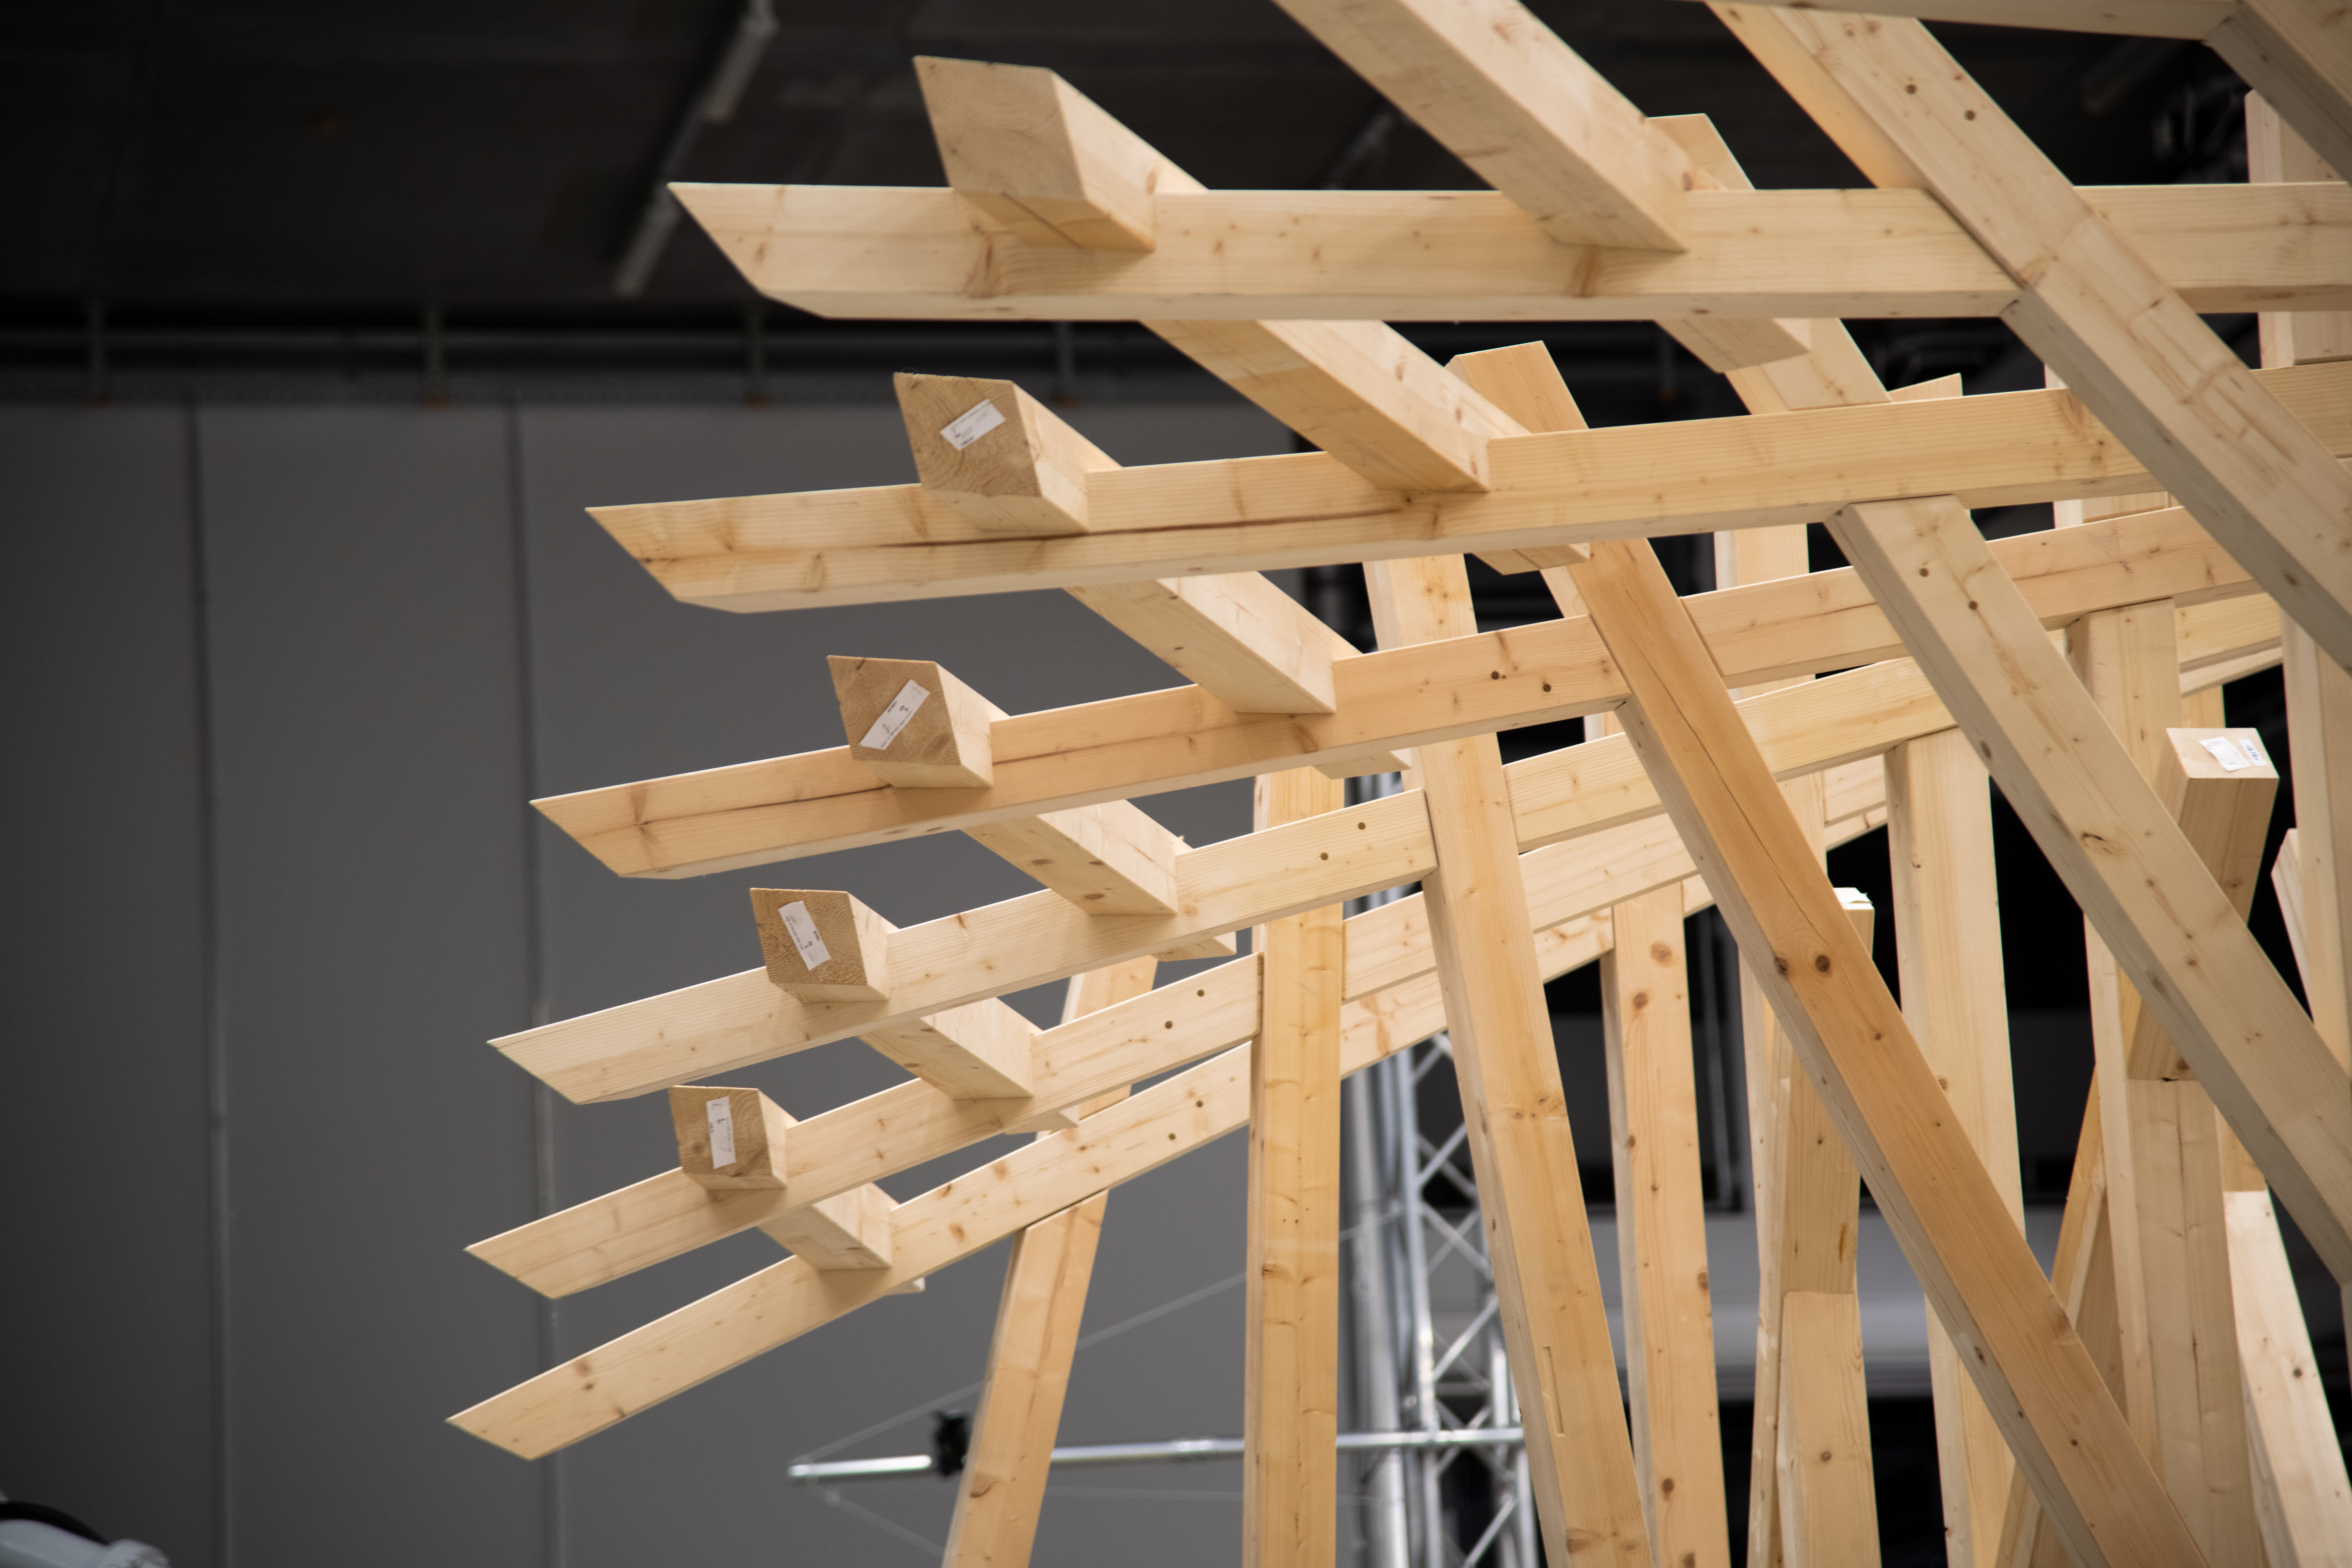
\includegraphics[width=15.92cm,height=10.62cm]{./images/image6.jpeg}
\end{figure}
}

The final segment bridges over Joint 5 and 6 and is connected to the tool changer. The images below show the attachment of the cable chain to the robotic quick changer a tangential configuration. A 3D-printed mounting piece (left drawing) was used to create an interface between the cable chain and one of the attachment flanges on the Schunk tool changer. The tangential layout prevents cable pinching even when Joint 5 is in a fully deflected position (see photo below, right). 

The combined effect of the retraction system pulling the cable chain, the swivel guide and the tangential layout allows the cable chain to move freely in almost all configurations. During the motion planning process, the joint range were limited to the following configurations (Joint 1 to 6):

{\footnotesize rm\_limits $=$ [(-175, 175), (-85, 145), (-175, 70), (-181, 181), (-120, 120), (-181, 181)]}

\begin{figure}[H]
\centering
\begin{subfigure}[b]{0.45\textwidth}
\centering
\includegraphics[width=\textwidth]{./images/image7.jpeg}
\end{subfigure}
\hfill
\begin{subfigure}[b]{0.45\textwidth}
\centering
\includegraphics[width=\textwidth]{./images/image8.jpeg}
\end{subfigure}
\end{figure}


\subsection{Collision Model}

The drawing below (left) shows the collision mesh (yellow) of the tool changer used for motion planning. Note that it covers a portion of volume where the cable chain leads out tangentially. The drawing below (right) shows the collision meshes of the forearm. Extra boxes (orange) can be seen covering the swivel guide location and the location where the cable chain would pass over the wrist.

\begin{figure}[H]
\centering
\begin{subfigure}[b]{0.45\textwidth}
\centering
\includegraphics[width=\textwidth]{./images/image9.jpeg}
\end{subfigure}
\hfill
\begin{subfigure}[b]{0.45\textwidth}
\centering
\includegraphics[width=\textwidth]{./images/image10.jpeg}
\end{subfigure}
\end{figure}


\subsection{Lessons Learnt}

One note regarding the \textbf{cable retraction length}. It was only after the implementation that the retraction length appears to be an issue. The combined motion range of Joint 4, 5 and 6 requires a larger retractable cable range than expected. The 500mm retraction range offered by the default Igus system is not sufficient. Extra slack sometimes remained in the system depending on the configuration. The image below shows the chain in a very loose state, this image was taken before the wrist swivel guide is installed. The situation improved slightly after it was installed. Note that for future implementation, a retraction length of 800mm to 1m is more appropriate.

\begin{figure}[H]
\includegraphics[width=14.33cm,height=7.11cm]{./images/image11.jpeg}
\end{figure}


\subsubsection{Design Software Implementation in Rhino Python}

The design software was upgraded from the previous Rhino (RH) Grasshopper (GH) implementation \textit{\textcolor[HTML]{B7B7B7}{(see \uline{5.5.1 Difficulty in interactive Modelling}) }}into a Python implementation within RH.

The main motivation is to depart from the GH functional programming paradigm, which automatically recomputes every downstream operation in the event of a data change. While this is a nice feature for ensuring all data is up to date, it also prevents any user interaction beyond changing the initial input. In addition, the full recomputation of every operation is slow and in many cases redundant.

The development to address this is a \textbf{model-based programming approach} that is focused on the creation and maintenance of a \textbf{Model}. Once created, this model can be revisited and edited. The diagram below shows the difference between (a) a functional programming paradigm and (b) a model-based approach.

\begin{figure}[H]
\includegraphics[width=8.59cm,height=4.42cm]{./images/image12.jpeg}
\end{figure}


The diagram below shows an example of some interactive assembly modelling functions that can benefit from the model-based approach. For example, the user can work between

\begin{itemize}
	\item (a) and (b) to change the beam arrangements

	\item (c) to resolve assembly direction problems

\end{itemize}
By updating only part of the model where it is necessary, the user decisions that were provided earlier can be kept. Note that it is not impossible but very difficult to achieve this with a GH script and its interface. By switching to Rhino Python, a different script can be used to handle each user interaction, and contain the intelligence on which part of the model needs updating.

\begin{figure}[H]
\includegraphics[width=13.98cm,height=10.71cm]{./images/image13.jpeg}
\end{figure}


The image below (left) shows the UI for editing the \textbf{assembly model}; commands such as AddBeam, Move Assemble, FlipBeamAssemblyDirection can be seen. The image below (right) shows the UI for editing the \textbf{assembly sequence}; commands such as MoveEarlier, MoveLater, PickElementToGoAfterThis, ChangeAssemblyMethod can be seen. In practice, I have found that the command FlipBeamAssemblyDirection is also helpful while editing the sequence.

\begin{figure}[H]
\centering
\begin{subfigure}[b]{0.45\textwidth}
\centering
\includegraphics[width=\textwidth]{./images/image14.jpeg}
\end{subfigure}
\hfill
\begin{subfigure}[b]{0.45\textwidth}
\centering
\includegraphics[width=\textwidth]{./images/image15.jpeg}
\end{subfigure}
\end{figure}


While there was no need to recreate the BusStop Assembly Model for this Dev Round, the newly developed process design workflow \textit{\textcolor[HTML]{B7B7B7}{(see the next section) }}benefited greatly from this improvement. The visualisation and interactive UI for process design is also accessible from the toolbar in Rhino. More screen capture can be found in the later sections \textit{\textcolor[HTML]{B7B7B7}{(see \uline{6.3.5.6 Process Visualization and Adjustment})}}.

\subsubsection{Process Design Workflow}

The process design workflow is a downstream operation after the Assembly Model is completed. In this thesis, it is conceived to be a human-in-the-loop workflow where a production engineer is present to bridge the gap between design and production. However, the thesis aims to study to what extent this step can be automated.

Because decisions made in this stage do not affect architectural and structural design results, this stage is referred to as\textbf{ Robotic Process Design} or \textbf{Process Design }in short. In this thesis, I call these software functions as Computer-Aided-Manufacturing (\textbf{CAM}) functions, as the counterpart of the CAD functions for Assembly Design.

The process design software follows the model-centric programming approach described in the previous section, including the following steps. Steps (3) to (5) are repeated as many times as necessary while the engineer makes changes.

\subsubsection{Creation of Process Model}

\begin{itemize}
\begin{itemize}
	\item The Process Model is created by combining the Assembly Model, Robot Model, Tool Models (Clamps, Docking Adapter and Grippers) and the Environment Model 

	\item Subsequent computation updates this Process Model

\end{itemize}
\end{itemize}
\subsection{Task Planning}

\begin{itemize}
\begin{itemize}
	\item A sequential list of High Level Assembly Tasks is computed using a flowchart method \textit{\textcolor[HTML]{B7B7B7}{(see 6.3.5.1 Task Planning with Flowchart)}}

	\item This list is expanded to a more comprehensive list of Low Level Tasks \textit{\textcolor[HTML]{B7B7B7}{(see 6.3.5.2 Expansion to Low Level Tasks)}}

\end{itemize}
	\item \textbf{Compute Process Parameters / Accept User Changes}

\begin{itemize}
	\item Process Parameters (such as Gripper and Clamp Choices) are computed based on the Assembly Model \textit{\textcolor[HTML]{B7B7B7}{(see 6.3.5.3 Process Parameters)}}

	\item Design rules are used to make decision automatically for parameters that have multiple options

	\item Parameters can be modified manually by the engineer if needed.

\end{itemize}
	\item \textbf{Compute Robot Targets and Object States}

\begin{itemize}
	\item Robot Targets are computed automatically for each Robot Motion \textit{\textcolor[HTML]{B7B7B7}{(see 6.3.5.4 Compute Robot Targets)}}

	\item Object States are computed automatically for each Keyframe between Tasks \textit{\textcolor[HTML]{B7B7B7}{(see 6.3.5.5 Compute Scene States)}}

\end{itemize}
	\item \textbf{Collision Detection and Keyframe Visualization}

\begin{itemize}
	\item Scene states can be used for automatic collision detection

	\item Engineer can identify difficult manoeuvres visually based on intuition \textit{\textcolor[HTML]{B7B7B7}{(see 6.3.5.6 Keyframe Visualization)}}

\end{itemize}
\end{itemize}
\section{Multimodal Motion Planning (MMMP)}

\begin{itemize}
\begin{itemize}
	\item Robotic Motions are planned sequentially, ensuring continuity between robot configurations \textit{\textcolor[HTML]{B7B7B7}{(see 6.3.5.7 Multimodal Motion Planning)}}

\end{itemize}
\end{itemize}
The diagram below shows the Process Design Workflow, the highlighted (grey) portion represents the initial creation of the Process Model, which is essentially a wrapper around all other important models. 

\begin{figure}[H]
\includegraphics[width=15.92cm,height=5.26cm]{./images/image16.jpeg}
\end{figure}


\begin{itemize}
	\item \textbf{Assembly Model} - Obtained from Assembly Design Phase, contains beams, joints and assembly sequence. \textit{\textcolor[HTML]{B7B7B7}{(see \uline{5.3.13 Assembly Model Data Structure and Functions})}}

	\item \textbf{Robot Model} - A comprehensive model that describes the geometry and kinematics of the robot. The implementation used is based on compas\_fab, that is based on URDF and SRDF formats used in ROS moveit! Planning framework \href{https://www.zotero.org/google-docs/?9FxuyJ}{(}\href{https://www.zotero.org/google-docs/?9FxuyJ}{\textit{Srdf - ROS Wiki}\href{https://www.zotero.org/google-docs/?9FxuyJ}{}, 2023; }\href{https://www.zotero.org/google-docs/?9FxuyJ}{\textit{Urdf - ROS Wiki}\href{https://www.zotero.org/google-docs/?9FxuyJ}{}, 2023)}.

	\item \textbf{Tool Models }- A model similar to the Robot Model. It is able to describe the geometry and kinematics of the tool. It also contains other parameters regarding how the tool can interact with timber beams and joints. The model is conceived to be prepared by the Tool Designer.

	\item \textbf{Construction Environment Model} - A geometrical model describing the static objects in the construction environment. The implementation in this thesis includes columns and floor of the laboratory, furniture and material stockpile. This model was constructed using a measuring probe from the iGPS system to measure the location of objects in the laboratory, and later modelling them using a rough representation. It shares the same frame of reference as the Robot Model. This approach has been used by other large scale projects in the past in the same laboratory \href{https://www.zotero.org/google-docs/?qIPEJd}{(Thoma et al., 2018)}.

\end{itemize}
Due to the complexity of the entire Process Design workflow, this section is long. This workflow diagram will be repeated as a guide in the beginning of each sub-sections to indicate (grey box) which step is being discussed.

\paragraph{Task Planning with Flowchart}

Task planning refers to the creation of a list of tasks to accomplish a goal. These tasks have been listed in \uline{6.1.1 DiRT Clamping Assembly Process Task List (v2)} using colloquial language.

\begin{figure}[H]
\includegraphics[width=15.92cm,height=5.12cm]{./images/image17.jpeg}
\end{figure}


In order to formalise the description such that it can be processed by a computer automatically. The flowchart planning method was developed for automating the creation of an assembly-task list according to the design specified in the Assembly Model \href{https://www.zotero.org/google-docs/?cKlfeU}{(Huang et al., 2021)}.

In the DiRT Clamping Assembly Process, different sets of assembly tasks are required depending on the number of joints a beam has with its neighbours. For example, the tools implemented in this round contains two gripper choices (PG1000 and PG1500) and two clamp choices (CL3 and CL3M). There are even more choices in later Dev Rounds. When combined, there are many possible combinations of gripper and clamps for each beam. For example,

\begin{itemize}
	\item Beam assembled with Gripper, placing on the ground platform, fixed manually. No clamps used.

	\item Beam assembled with Gripper holding it and Clamp(s) clamping it to neighbouring beams at the shared joints.

\begin{itemize}
	\item Gripper + One clamp

	\item Gripper + Two clamps

	\item Gripper + Three clamps

	\item Gripper + Four clamps (not used in the BusStop design)

\end{itemize}
\end{itemize}
In order to be flexible for planning different scenarios and be generalizable for later development, the flowchart method uses \textbf{loops }and \textbf{conditionals }to plan the tasks. The following diagram shows the flowchart used for planning the BusStop. It consists of a global loop (a) that iterates through each beam to be assembled, and two other loops (b) and (c) that iterates through the required clamps for the operations. A conditional (d) is used to decide whether the assembly requires synchronised clamping. Whenever the flowchart encounters a \textbf{Task}, that task is added to a \textbf{Task List}. 

\begin{figure}[H]
\includegraphics[width=15.92cm,height=10.69cm]{./images/image18.jpeg}
\end{figure}


Note that there are some variables used in the flowchart, they consist of \textbf{Assembly Model Parameters} and \textbf{Process Model Parameters}. At the beginning of this process design phase, the assembly motion parameters can be extracted from the Assembly Model but the process model parameters have not been computed yet. Therefore these parameters are left as a variable, the values of which can be binded later \textit{\textcolor[HTML]{B7B7B7}{(see section \uline{6.3.5.2 Process Parameters)}}}. This late binding technique is commonly used in TAMP context \href{https://www.zotero.org/google-docs/?svi3ss}{(Garrett et al., 2021a; Lozano-Pérez $\&$ Kaelbling, 2014)}.

\begin{table}[H]
\begin{adjustbox}{max width=\textwidth}
\begin{tabular}{p{7.91cm}p{7.97cm}}
\hline
\multicolumn{1}{|p{7.91cm}}{{\footnotesize \textbf{Assembly Model Parameters Required}}} & 
\multicolumn{1}{|p{7.97cm}|}{{\footnotesize \textbf{Process Model Parameters Required}}} \\ 
\hline
\multicolumn{1}{|p{7.91cm}}{{\footnotesize Fixed from the previous Assembly Design Phase}} & 
\multicolumn{1}{|p{7.97cm}|}{{\footnotesize Computed or chosen later in the next steps}} \\ 
\hline
\multicolumn{1}{|p{7.91cm}}{{\footnotesize \textbf{Assembly Sequence:}} \newline
{\footnotesize \textbf{bid }$=$ beam\_id $=$ assembly\_sequence[i]} \newline
{\footnotesize     where: i $=$ integer iterator} \newline
{\footnotesize beam $=$ assembly.beams[bid]} \newline
{\footnotesize     where: type(assembly) $=$ Assembly} \newline
{\footnotesize     where: type(beam) $=$ Beam} \newline
{\footnotesize \textbf{Joints and Neighbours:}} \newline
{\footnotesize \textbf{jid }$=$ joint\_id $=$ beam.joints\_to\_assemble[j] } \newline
{\footnotesize     where: j $=$ integer iterator} \newline
{\footnotesize     decomposing: jid $=$ (bid, nid)} \newline
{\footnotesize     where: nid $=$ neighbour\_beam\_id}} & 
\multicolumn{1}{|p{7.97cm}|}{{\footnotesize \textbf{Tool Choice:}} \newline
{\footnotesize \textbf{cid }$=$ clamp\_id $=$ beam.clamp\_on\_joint[jid]} \newline
{\footnotesize \textbf{gid }$=$ gripper\_id $=$ beam.gripper\_choice}} \\ 
\hline
\end{tabular}
\end{adjustbox}
\end{table}
\paragraph{Expanding Task Groups}

The list of tasks planned by the flowchart method is considered \textbf{High-Level Tasks }or \textbf{Task Groups}. Each of which can be expanded to a list of \textbf{Low-Level Tasks} that are directly related to the functions provided by the L2 and L3 controllers \textit{\textcolor[HTML]{B7B7B7}{(see 5.2.4 Distributed Control System)}}. The following table lists all the low-level tasks used in this development round and the \textbf{Task Agents }(including the human operator) and Controller that are responsive for their execution.

\begin{table}[H]
\begin{adjustbox}{max width=\textwidth}
\begin{tabular}{p{2.46cm}p{2.33cm}p{11.11cm}}
\hline
\multicolumn{1}{|p{2.46cm}}{{\footnotesize \textbf{Task Agents}}} & 
\multicolumn{1}{|p{2.33cm}}{{\footnotesize \textbf{Controller}}} & 
\multicolumn{1}{|p{11.11cm}|}{{\footnotesize \textbf{Low Level Task Available }}} \\ 
\hline
\multicolumn{1}{|p{2.46cm}}{{\footnotesize RFL Robot}} & 
\multicolumn{1}{|p{2.33cm}}{{\footnotesize L2 ROS RRC Driver for RFL Robot}} & 
\multicolumn{1}{|p{11.11cm}|}{\begin{itemize}
	\item {\footnotesize \textbf{Linear Motion (LM)}} \newline
	\item {\footnotesize \textbf{Free Motion (FM)}} \newline
{\footnotesize (refer to \uline{5.2.7.3 Motion Planner} and \uline{5.2.8 Executing Robotic Motion})}} \\ 
\hline
\multicolumn{1}{|p{2.46cm}}{{\footnotesize Clamp}} & 
\multicolumn{1}{|p{2.33cm}}{{\footnotesize L2 Clamp Controller}} & 
\multicolumn{1}{|p{11.11cm}|}{	\item {\footnotesize \textbf{Clamp Jaw Motion}} \newline
{\footnotesize (refer to \uline{4.3.1 Lap Clamp CL1 - Proof of Concept})} \newline
{\footnotesize (refer to \uline{5.3.4 Lap Clamp CL3 Hardware})}} \\ 
\hline
\multicolumn{1}{|p{2.46cm}}{{\footnotesize RFL Robots and Clamp(s)}} & 
\multicolumn{1}{|p{2.33cm}}{{\footnotesize L3 Process Controller}} & 
\multicolumn{1}{|p{11.11cm}|}{	\item {\footnotesize \textbf{Clamp and Robot Sync Linear Motion (SM)}} \newline
{\footnotesize (refer to \uline{5.2.3 Synchronisation between Clamp and RFL Robot})}} \\ 
\hline
\multicolumn{1}{|p{2.46cm}}{{\footnotesize Clamp}} & 
\multicolumn{1}{|p{2.33cm}}{\multirow{3}{*}{\parbox{2.33cm}{{\footnotesize L2 ROS RRC Driver for RFL Robot} \newline
{\footnotesize (Digital IO)}}}} & 
\multicolumn{1}{|p{11.11cm}|}{	\item {\footnotesize \textbf{Open attachment gripper}} \newline
	\item {\footnotesize \textbf{Close attachment gripper}} \newline
{\footnotesize (refer to \uline{4.3.1.2 Gripper for Hanging Clamp})}} \\ 
\hhline{-~-}
\multicolumn{1}{|p{2.46cm}}{{\footnotesize Parallel Gripper}} & 
\multicolumn{1}{|p{2.33cm}}{\end{itemize}
} & 
\multicolumn{1}{|p{11.11cm}|}{\begin{itemize}
	\item {\footnotesize \textbf{Open Gripper}} \newline
	\item {\footnotesize \textbf{Close Gripper}} \newline
{\footnotesize (refer to \uline{5.3.6 Parallel Gripper PG500 and PG1000})}} \\ 
\hhline{-~-}
\multicolumn{1}{|p{2.46cm}}{{\footnotesize Docking Adapter}} & 
\multicolumn{1}{|p{2.33cm}}{\end{itemize}
} & 
\multicolumn{1}{|p{11.11cm}|}{\begin{itemize}
	\item {\footnotesize \textbf{Lock Tool}} \newline
	\item {\footnotesize \textbf{Unlock Tool}} \newline
{\footnotesize (refer to \uline{5.3.5 Docking adapter})}} \\ 
\hline
\multicolumn{1}{|p{2.46cm}}{{\footnotesize Operator}} & 
\multicolumn{1}{|p{2.33cm}}{{\footnotesize Operator}} & 
\multicolumn{1}{|p{11.11cm}|}{	\item {\footnotesize \textbf{Place Beams from Storage in Robot Gripper}} \newline
\end{itemize}
{\footnotesize (refer to \uline{5.1.1 Scope for the First Large-Scale Demonstration})}} \\ 
\hline
\end{tabular}
\end{adjustbox}
\end{table}
\vspace{2\baselineskip}
Note the following properties:

\begin{itemize}
	\item Only \textbf{LM}, \textbf{FM }and \textbf{SM }require motion planning. 

	\item Clamp and Robot Sync Linear Motion (SM) is provided by the L3 controller as it requires the coordination of the L2 Clamp Controller and the L2 ROS RRC Driver. 

	\item Other L2 tasks are also executed through the L3 Process Controller because it provides flow control \textit{\textcolor[HTML]{B7B7B7}{(see \uline{5.3.15 Process Execution Controller})}}. 

The diagram below shows all the task groups used in this development round expanded into its constituting low-level tasks. Those that are marked with ``TC" means that a Taught Configuration was used for its target pose.

\begin{figure}[H]
\includegraphics[width=14.0cm,height=2.7cm]{./images/image19.jpeg}
\caption{Only LM, FM and SM require motion planning. $\bullet$ Clamp and Robot Sync Linear Motion (SM) is provided by the L3 controller as it requires the coordination of the L2 Clamp Controller and the L2 ROS RRC Driver. $\bullet$ Other L2 tasks are also executed through the L3 Process Controller because it provides flow control (see 5.3.15 Process Execution Controller). $\bullet$ Clamp, Gripper, and Docking Adapter pneumatic actuators are controlled by the L2 ROS RRC Driver because the pneumatic valves are controlled over the RFL robot's network. The compressed air for the clamp and gripper passes through the docking adapter.}
\label{fig:only_lm_fm_and_sm}
\end{figure}


\begin{figure}[H]
\includegraphics[width=15.92cm,height=15.49cm]{./images/image20.jpeg}
\end{figure}


\begin{figure}[H]
\includegraphics[width=15.92cm,height=10.72cm]{./images/image21.jpeg}
\end{figure}


\begin{figure}[H]
\includegraphics[width=15.92cm,height=7.37cm]{./images/image22.jpeg}
\end{figure}


\end{itemize}
\vspace{1\baselineskip}
\begin{figure}[H]
\includegraphics[width=7.0cm,height=10.78cm]{./images/image23.jpeg}
\end{figure}


\vspace{1\baselineskip}
There are some useful techniques for designing the Low Level Tasks. 

\begin{itemize}
	\item \textbf{Start with Free Motion} - Notice that all the High Level Tasks start with a Free Motion. This essentially means bringing the robot from wherever it was to this specific target at the beginning of this motion. This effectively allows the High Level Tasks to be decoupled from each other, allowing them to be modular and reusable within the flowchart.

	\item \textbf{Use Approach as First Target} - The target of the first free motion is often set at a small distance away from the actual target of interest. For example, in ‘PickClampFromStorage’, the robot is programmed to first arrive at an ‘approach’ point before moving linearly to insert the docking adapter into the tool-side. This gives the free motion planner (FMP) more ‘room’ for planning the trajectory and results in shorter planning time.

	\item \textbf{Use Retract as Last Target} - Similar to the approach point, the retract point allows the robot to move freely away to the next task.

	\item \textbf{Use Linear Move for Narrow Passages} - The use of linear move can also help to explicitly define how the robot moves through a narrow gap. This is called the Narrow Passage problem in the field of motion planning. In the ‘PlaceClampToStructure’, the robot needs to slot the clamp around a timber beam where the hanging jaw is only slightly larger than the beam. The explicit use of two linear motions reduces the guesswork needed by the motion planner which results in shorter planning time.

	\item \textbf{Split Motions for changing Allowable Collision Matrix (ACM)} - Whenever the robot is making or breaking contact during the process, a different ACM is needed for planning purposes. For example in ‘AssembleBeamWithClamps’, the first free motion should not allow the active beam to collide with the clamps. However, in the subsequent linear move where the beam is placed into the clamp jaws, the ACM must allow this contact. Because each motion planning call can only support a fixed ACM, therefore an ACM change can be achieved by splitting the motion.

\end{itemize}
The following diagram shows the planned \textbf{Task List} for assembling a beam that requires two clamps. Notice the total number of Low Level Tasks involved and the use of the high level tasks to make designing them easier.

\begin{figure}[H]
\includegraphics[width=13.01cm,height=13.08cm]{./images/image24.jpeg}
\end{figure}


\paragraph{Process Parameters}

After the task list is completed, the next task is to compute the process parameters. Process parameters refers to all the parameters that are necessary to compute the details of the assembly process, such as Robotic Targets.

\begin{figure}[H]
\includegraphics[width=15.92cm,height=5.19cm]{./images/image25.jpeg}
\end{figure}


The table below shows the most important process parameters used for the clamped assembly process, the first column lists the 1:1 relationship, and how the parameters are related to the models. For example, there is only one ``Assembly Sequence" in the whole Assembly Model, but there is one ``Designed Location" for every beam.

The second column lists the design phase where the values are generated. This can be Assembly Design (\textbf{AD}), Process Design (\textbf{PD}) and Tool Design (\textbf{TD}). In this PD phase, the production engineer’s role is to select suitable PD parameters such that the robotic process can be carried out. 

The third column lists the domain expert involved in deciding the values. This can be Architectural and Structural Designer (\textbf{ASD}), Process Engineer (\textbf{PE}) and Tool Engineer (\textbf{TE}). It can also be Automatic Algorithms (Auto) that are used to infer the parameters from other parameters. In cases where the inference result has multiple possibilities, rule-based logic can be used for automatically making the selection. If necessary, the production engineer can also make adjustments to the selection.

\begin{table}[H]
\begin{adjustbox}{max width=\textwidth}
\begin{tabular}{p{2.09cm}p{1.51cm}p{1.93cm}p{5.92cm}p{4.48cm}}
\hline
\multicolumn{1}{|p{2.09cm}}{{\footnotesize \textbf{Relation Level}}} & 
\multicolumn{1}{|p{1.51cm}}{{\footnotesize \textbf{Design Phase}}} & 
\multicolumn{1}{|p{1.93cm}}{{\footnotesize \textbf{Designer}}} & 
\multicolumn{1}{|p{5.92cm}}{{\footnotesize \textbf{Description}}} & 
\multicolumn{1}{|p{4.48cm}|}{{\footnotesize \textbf{Data Type}}} \\ 
\hline
\multicolumn{1}{|p{2.09cm}}{\multirow{3}{*}{\parbox{2.09cm}{{\footnotesize Process}}}} & 
\multicolumn{1}{|p{1.51cm}}{{\footnotesize TD}} & 
\multicolumn{1}{|p{1.93cm}}{{\footnotesize TE}} & 
\multicolumn{1}{|p{5.92cm}}{{\footnotesize Robot Model}} & 
\multicolumn{1}{|p{4.48cm}|}{{\footnotesize Robot Model}} \\ 
\hhline{~----}
\multicolumn{1}{|p{2.09cm}}{} & 
\multicolumn{1}{|p{1.51cm}}{{\footnotesize \textbf{PD}}} & 
\multicolumn{1}{|p{1.93cm}}{{\footnotesize \textbf{PE}}} & 
\multicolumn{1}{|p{5.92cm}}{{\footnotesize Environment Models}} & 
\multicolumn{1}{|p{4.48cm}|}{{\footnotesize 3D Geometry}} \\ 
\hhline{~----}
\multicolumn{1}{|p{2.09cm}}{} & 
\multicolumn{1}{|p{1.51cm}}{{\footnotesize \textbf{PD}}} & 
\multicolumn{1}{|p{1.93cm}}{{\footnotesize \textbf{PE}}} & 
\multicolumn{1}{|p{5.92cm}}{{\footnotesize Position of Assembly Model relative to the Robot }} & 
\multicolumn{1}{|p{4.48cm}|}{{\footnotesize T [World Frame]}} \\ 
\hline
\multicolumn{1}{|p{2.09cm}}{\multirow{2}{*}{\parbox{2.09cm}{{\footnotesize Assembly}}}} & 
\multicolumn{1}{|p{1.51cm}}{{\footnotesize AD}} & 
\multicolumn{1}{|p{1.93cm}}{{\footnotesize DE / PE}} & 
\multicolumn{1}{|p{5.92cm}}{{\footnotesize Assembly Sequence}} & 
\multicolumn{1}{|p{4.48cm}|}{{\footnotesize List of Beam ID}} \\ 
\hhline{~----}
\multicolumn{1}{|p{2.09cm}}{} & 
\multicolumn{1}{|p{1.51cm}}{{\footnotesize AD}} & 
\multicolumn{1}{|p{1.93cm}}{{\footnotesize Auto}} & 
\multicolumn{1}{|p{5.92cm}}{{\footnotesize Beam Connectivity}} & 
\multicolumn{1}{|p{4.48cm}|}{{\footnotesize Graph of Beams and Joints}} \\ 
\hline
\multicolumn{1}{|p{2.09cm}}{\multirow{8}{*}{\parbox{2.09cm}{{\footnotesize Beam}}}} & 
\multicolumn{1}{|p{1.51cm}}{{\footnotesize AD}} & 
\multicolumn{1}{|p{1.93cm}}{{\footnotesize DE}} & 
\multicolumn{1}{|p{5.92cm}}{{\footnotesize Designed Location}} & 
\multicolumn{1}{|p{4.48cm}|}{{\footnotesize T [World Frame]}} \\ 
\hhline{~----}
\multicolumn{1}{|p{2.09cm}}{} & 
\multicolumn{1}{|p{1.51cm}}{{\footnotesize AD}} & 
\multicolumn{1}{|p{1.93cm}}{{\footnotesize DE}} & 
\multicolumn{1}{|p{5.92cm}}{{\footnotesize Assembly Direction}} & 
\multicolumn{1}{|p{4.48cm}|}{{\footnotesize T [Beam Frame]}} \\ 
\hhline{~----}
\multicolumn{1}{|p{2.09cm}}{} & 
\multicolumn{1}{|p{1.51cm}}{{\footnotesize \textbf{PD}}} & 
\multicolumn{1}{|p{1.93cm}}{{\footnotesize \textbf{PE }/ Auto}} & 
\multicolumn{1}{|p{5.92cm}}{{\footnotesize Gripper Choice}} & 
\multicolumn{1}{|p{4.48cm}|}{{\footnotesize Gripper ID}} \\ 
\hhline{~----}
\multicolumn{1}{|p{2.09cm}}{} & 
\multicolumn{1}{|p{1.51cm}}{{\footnotesize \textbf{PD}}} & 
\multicolumn{1}{|p{1.93cm}}{{\footnotesize \textbf{PE }/ Auto}} & 
\multicolumn{1}{|p{5.92cm}}{{\footnotesize Grasp Face}} & 
\multicolumn{1}{|p{4.48cm}|}{{\footnotesize Face ID}} \\ 
\hhline{~----}
\multicolumn{1}{|p{2.09cm}}{} & 
\multicolumn{1}{|p{1.51cm}}{{\footnotesize \textbf{PD}}} & 
\multicolumn{1}{|p{1.93cm}}{{\footnotesize \textbf{PE }/ Auto}} & 
\multicolumn{1}{|p{5.92cm}}{{\footnotesize Grasp Position}} & 
\multicolumn{1}{|p{4.48cm}|}{{\footnotesize Length along beam}} \\ 
\hhline{~----}
\multicolumn{1}{|p{2.09cm}}{} & 
\multicolumn{1}{|p{1.51cm}}{{\footnotesize \textbf{PD}}} & 
\multicolumn{1}{|p{1.93cm}}{{\footnotesize Auto}} & 
\multicolumn{1}{|p{5.92cm}}{{\footnotesize Grasp Pose}} & 
\multicolumn{1}{|p{4.48cm}|}{{\footnotesize Inverse T [Beam Frame]}} \\ 
\hhline{~----}
\multicolumn{1}{|p{2.09cm}}{} & 
\multicolumn{1}{|p{1.51cm}}{{\footnotesize \textbf{PD}}} & 
\multicolumn{1}{|p{1.93cm}}{{\footnotesize Auto}} & 
\multicolumn{1}{|p{5.92cm}}{{\footnotesize Beam Pickup Location}} & 
\multicolumn{1}{|p{4.48cm}|}{{\footnotesize T [World Frame]}} \\ 
\hhline{~----}
\multicolumn{1}{|p{2.09cm}}{} & 
\multicolumn{1}{|p{1.51cm}}{{\footnotesize \textbf{PD}}} & 
\multicolumn{1}{|p{1.93cm}}{{\footnotesize Auto}} & 
\multicolumn{1}{|p{5.92cm}}{{\footnotesize Clamp Jaw Approach Direction} \newline
{\scriptsize (only for beams that require clamps)}} & 
\multicolumn{1}{|p{4.48cm}|}{{\footnotesize T [World Frame]}} \\ 
\hline
\multicolumn{1}{|p{2.09cm}}{\multirow{7}{*}{\parbox{2.09cm}{{\footnotesize Joint}}}} & 
\multicolumn{1}{|p{1.51cm}}{{\footnotesize AD}} & 
\multicolumn{1}{|p{1.93cm}}{{\footnotesize Auto}} & 
\multicolumn{1}{|p{5.92cm}}{{\footnotesize Joint Position}} & 
\multicolumn{1}{|p{4.48cm}|}{{\footnotesize T [Beam Frame]}} \\ 
\hhline{~----}
\multicolumn{1}{|p{2.09cm}}{} & 
\multicolumn{1}{|p{1.51cm}}{{\footnotesize TD}} & 
\multicolumn{1}{|p{1.93cm}}{{\footnotesize TE}} & 
\multicolumn{1}{|p{5.92cm}}{{\footnotesize Allowable Clamp Choices}} & 
\multicolumn{1}{|p{4.48cm}|}{} \\ 
\hhline{~----}
\multicolumn{1}{|p{2.09cm}}{} & 
\multicolumn{1}{|p{1.51cm}}{{\footnotesize \textbf{PD}}} & 
\multicolumn{1}{|p{1.93cm}}{{\footnotesize \textbf{PE }/ Auto}} & 
\multicolumn{1}{|p{5.92cm}}{{\footnotesize Clamp Choice}} & 
\multicolumn{1}{|p{4.48cm}|}{{\footnotesize Clamp Type}} \\ 
\hhline{~----}
\multicolumn{1}{|p{2.09cm}}{} & 
\multicolumn{1}{|p{1.51cm}}{{\footnotesize \textbf{PD}}} & 
\multicolumn{1}{|p{1.93cm}}{{\footnotesize Auto}} & 
\multicolumn{1}{|p{5.92cm}}{{\footnotesize Assigned Clamp Device}} & 
\multicolumn{1}{|p{4.48cm}|}{{\footnotesize Clamp ID}} \\ 
\hhline{~----}
\multicolumn{1}{|p{2.09cm}}{} & 
\multicolumn{1}{|p{1.51cm}}{{\footnotesize TD}} & 
\multicolumn{1}{|p{1.93cm}}{{\footnotesize TE}} & 
\multicolumn{1}{|p{5.92cm}}{{\footnotesize Allowable Clamp Attach Poses}} & 
\multicolumn{1}{|p{4.48cm}|}{{\footnotesize T [Joint Frame]}} \\ 
\hhline{~----}
\multicolumn{1}{|p{2.09cm}}{} & 
\multicolumn{1}{|p{1.51cm}}{{\footnotesize \textbf{PD}}} & 
\multicolumn{1}{|p{1.93cm}}{{\footnotesize \textbf{PE }/ Auto}} & 
\multicolumn{1}{|p{5.92cm}}{{\footnotesize Clamp Attach Pose}} & 
\multicolumn{1}{|p{4.48cm}|}{{\footnotesize T [Joint Frame]}} \\ 
\hhline{~----}
\multicolumn{1}{|p{2.09cm}}{} & 
\multicolumn{1}{|p{1.51cm}}{{\footnotesize AD}} & 
\multicolumn{1}{|p{1.93cm}}{{\footnotesize Auto}} & 
\multicolumn{1}{|p{5.92cm}}{{\footnotesize Allowable Assembly Direction}} & 
\multicolumn{1}{|p{4.48cm}|}{{\footnotesize T [Joint Frame]}} \\ 
\hline
\multicolumn{1}{|p{2.09cm}}{\multirow{3}{*}{\parbox{2.09cm}{{\footnotesize All DiRT Tools \\ (Gripper and Clamps)}}}} & 
\multicolumn{1}{|p{1.51cm}}{{\footnotesize \textbf{PD}}} & 
\multicolumn{1}{|p{1.93cm}}{{\footnotesize \textbf{PE}}} & 
\multicolumn{1}{|p{5.92cm}}{{\footnotesize Storage Location (Tool Storage Station)}} & 
\multicolumn{1}{|p{4.48cm}|}{{\footnotesize T [World Frame]}} \\ 
\hhline{~----}
\multicolumn{1}{|p{2.09cm}}{} & 
\multicolumn{1}{|p{1.51cm}}{{\footnotesize TM}} & 
\multicolumn{1}{|p{1.93cm}}{{\footnotesize TE}} & 
\multicolumn{1}{|p{5.92cm}}{{\footnotesize Storage Retract Direction}} & 
\multicolumn{1}{|p{4.48cm}|}{{\footnotesize T [Tool Base Frame]}} \\ 
\hhline{~----}
\multicolumn{1}{|p{2.09cm}}{} & 
\multicolumn{1}{|p{1.51cm}}{{\footnotesize TM}} & 
\multicolumn{1}{|p{1.93cm}}{{\footnotesize TE}} & 
\multicolumn{1}{|p{5.92cm}}{{\footnotesize Kinematic Chain Link FK }} & 
\multicolumn{1}{|p{4.48cm}|}{{\footnotesize T [Tool Base Frame]}} \\ 
\hline
\multicolumn{1}{|p{2.09cm}}{\multirow{2}{*}{\parbox{2.09cm}{{\footnotesize Clamp}}}} & 
\multicolumn{1}{|p{1.51cm}}{{\footnotesize TM}} & 
\multicolumn{1}{|p{1.93cm}}{{\footnotesize TE}} & 
\multicolumn{1}{|p{5.92cm}}{{\footnotesize Beam-Approach-Jaw Direction }} & 
\multicolumn{1}{|p{4.48cm}|}{{\footnotesize T [Tool Base Frame]}} \\ 
\hhline{~----}
\multicolumn{1}{|p{2.09cm}}{} & 
\multicolumn{1}{|p{1.51cm}}{{\footnotesize TM}} & 
\multicolumn{1}{|p{1.93cm}}{{\footnotesize TE}} & 
\multicolumn{1}{|p{5.92cm}}{{\footnotesize Clamp-Attach-To-Beam Direction (x2 steps)}} & 
\multicolumn{1}{|p{4.48cm}|}{{\footnotesize T [Tool Base Frame]}} \\ 
\hline
\multicolumn{1}{|p{2.09cm}}{\multirow{3}{*}{\parbox{2.09cm}{{\footnotesize Gripper}}}} & 
\multicolumn{1}{|p{1.51cm}}{{\footnotesize TM}} & 
\multicolumn{1}{|p{1.93cm}}{{\footnotesize TE}} & 
\multicolumn{1}{|p{5.92cm}}{{\footnotesize Gripper-Approach-Beam Direction}} & 
\multicolumn{1}{|p{4.48cm}|}{{\footnotesize T [Tool Base Frame]}} \\ 
\hhline{~----}
\multicolumn{1}{|p{2.09cm}}{} & 
\multicolumn{1}{|p{1.51cm}}{{\footnotesize \textbf{PD}}} & 
\multicolumn{1}{|p{1.93cm}}{{\footnotesize \textbf{PE}}} & 
\multicolumn{1}{|p{5.92cm}}{{\footnotesize Gripper Location for Beam Pickup}} & 
\multicolumn{1}{|p{4.48cm}|}{{\footnotesize T [World Frame]}} \\ 
\hhline{~----}
\multicolumn{1}{|p{2.09cm}}{} & 
\multicolumn{1}{|p{1.51cm}}{{\footnotesize \textbf{PD}}} & 
\multicolumn{1}{|p{1.93cm}}{{\footnotesize \textbf{PE }/ Auto}} & 
\multicolumn{1}{|p{5.92cm}}{{\footnotesize Beam Pickup Retract Direction}} & 
\multicolumn{1}{|p{4.48cm}|}{{\footnotesize T [World Frame]}} \\ 
\hline
\multicolumn{1}{|p{2.09cm}}{\multirow{2}{*}{\parbox{2.09cm}{{\footnotesize Docking Adapter}}}} & 
\multicolumn{1}{|p{1.51cm}}{{\footnotesize TM}} & 
\multicolumn{1}{|p{1.93cm}}{{\footnotesize TE}} & 
\multicolumn{1}{|p{5.92cm}}{{\footnotesize Dock Approach Direction}} & 
\multicolumn{1}{|p{4.48cm}|}{{\footnotesize T [Adapter Base Frame]}} \\ 
\hhline{~----}
\multicolumn{1}{|p{2.09cm}}{} & 
\multicolumn{1}{|p{1.51cm}}{{\footnotesize TM}} & 
\multicolumn{1}{|p{1.93cm}}{{\footnotesize TE}} & 
\multicolumn{1}{|p{5.92cm}}{{\footnotesize Tool Link FK }} & 
\multicolumn{1}{|p{4.48cm}|}{{\footnotesize T [Adapter Base Frame]}} \\ 
\hline
\end{tabular}
\end{adjustbox}
\end{table}
\vspace{24\baselineskip}
{\scriptsize $\ast$ T $=$ Transformation Data Type, value in the bracket is the transformation’s base frame.}

The following three parameters regarding the parallel gripper is an example where parameter values were computed using rule-based logic. This is applied as the initial values before the production engineer reviews them:

\begin{itemize}
	\item \textbf{Gripper Choice }- The decision between the shorter PG500 and longer PG1000 can be made based on the length of the beam, the threshold was set at 1200mm.

	\item \textbf{Grasp Face} - The grasp face was selected such that the gripper faced downwards during assembly. For vertical columns, the gripper was chosen to face the centre of the structure.

	\item \textbf{Grasp Position} - The centre of the beam was used as default. 

\end{itemize}
Based on the three parameters, the \textbf{Grasp Pose} (a transformation that relates between Gripper Grasp Frame and Beam Base Frame) is automatically computed. Note that there are numerous grasp pose possibilities. However, most of them are not viable because of collisions with the structure or the clamps. Nevertheless, this rule set was designed to maximise the chance of selecting a viable solution and helped reduce the work needed when the production engineer reviews them and makes changes to them. 

The set of images below shows the interface for the production engineer to select the gripper parameters. Specifically, four different Grasp Face decisions are shown. Note that only one of them is viable because the others have collisions (highlighted in orange). 

\begin{figure}[H]
\centering
\begin{subfigure}[b]{0.23\textwidth}
\centering
\includegraphics[width=\textwidth]{./images/image26.jpeg}
\end{subfigure}
\hfill
\begin{subfigure}[b]{0.23\textwidth}
\centering
\includegraphics[width=\textwidth]{./images/image27.jpeg}
\end{subfigure}
\hfill
\begin{subfigure}[b]{0.23\textwidth}
\centering
\includegraphics[width=\textwidth]{./images/image28.jpeg}
\end{subfigure}
\hfill
\begin{subfigure}[b]{0.23\textwidth}
\centering
\includegraphics[width=\textwidth]{./images/image29.jpeg}
\end{subfigure}
\end{figure}


Theoretically, a more advanced method would be to search the three parametric dimensions automatically to find a solution where the gripper does not cause collision. Additionally, it would be ideal to select a grasp position as close to the centre as possible to reduce imbalance. However, such algorithms were not implemented in the development because human intuition can often identify the solution fairly quickly. 

\paragraph{Compute Robot Targets}

\textbf{Robot target }refers to the goal pose of the robotic flange in each Robotic Motion (Linear and Free Motion) in the planned task list. It is also called the \textbf{Robot Flange Frame}, \textbf{Robot Frame}, or \textbf{Target Pose} depending on the context. 

As seen earlier in the expanded low level task list, the assembly of one beam contains many robot motions and the whole assembly contains many more. Because of the non-repetitive geometry and position of the beams in the assembly design, the targets for each motion are mostly unique. Furthermore, the targets have to be recomputed for visualisation whenever the process parameters are changed. For example, when the process engineer reviews the robotic tasks. Therefore it is important to have an automated system to compute the targets to ensure an efficient Process Design workflow.

Although it may not be obvious, all the concepts covered in the previous sections, such as the Assembly Model, Tool Models, Tasks, Task List, Process Parameters, are all designed in preparation for this computation step. 

\begin{figure}[H]
\includegraphics[width=15.92cm,height=5.19cm]{./images/image30.jpeg}
\end{figure}


\vspace{1\baselineskip}
\subsection{Kinematic Chain}

The first step to understand this computation is to introduce the concept of the \textbf{Kinematic Chain} of a robotic system \href{https://www.zotero.org/google-docs/?LgUOmG}{(LaValle, 2006)}. The kinematic chain refers to the chain of components attached to the flange of the robot, such as the Docking Adapter, Grippers and Beams. These components are represented by their corresponding models and are connected in a chain. The diagram below shows the kinematic chain when the robot is holding a beam in the gripper. 

\begin{figure}[H]
\includegraphics[width=15.92cm,height=8.18cm]{./images/image31.jpeg}
\end{figure}


The coloured boxes represent the computational models of the components in the chain and contain properties that describe them. They have \textbf{intrinsic properties}, values of which do not change during the process, and \textbf{extrinsic properties}, values of which can be changed by task agents. For example, the pose (a.k.a. Frame) of a Gripper is an extrinsic prosperity because it is changed when it is moved around. 

The column on the left of the models shows the kinematic relationship between the pose of each object. Notice how they are related in a chain-like arrangement. Every component contains a base frame and a child frame. The geometrical relationship between the two is a \textbf{transformation function} \textbf{(T) }that can be extracted from the models. If this transformation function is defined as an intrinsic property of the component models, they can have a known and fixed value. Which means that as long as one of the frames in this frame is known, all the other frames in the chain can be computed, including the Robot Target at the top. On the right side of the diagram, is a flowchart that shows the application of the transformation to compute the up-chain or down-chain neighbours, once a single frame can be determined.

Note that the Grasp Pose is modelled as a component in the chain, even though it does not have a physical existence. This is because the grasp pose for each beam is variable from beam to beam, by treating it as a separate object that is created during Process Design, it avoids the complication of managing a changing transformation function in the Gripper Model.

\subsection{Kinematic Switch}

The second important concept is that the kinematic chain can change during the assembly process whenever the robot is making or breaking contact with objects. For example, when picking up a beam or letting it go. The change in the kinematic chain is referred to as a \textbf{Kinematic Switch} \href{https://www.zotero.org/google-docs/?QSVbB7}{(Garrett et al., 2021b)}. 

The following diagram shows all the possible kinematic chain arrangements used during the DiRT clamping assembly process. These arrangements are called \textbf{modes }in MMMP. The bottom row of the diagram shows how the modes are switched between each other during the high-level tasks mentioned earlier \textit{\textcolor[HTML]{B7B7B7}{(see 6.3.5.1 Task Planning with Flowchart)}}. 

Note that some of the high level tasks can have more than one kinematic switch, and some can have none. It is just a coincidence that the tasks used in the clamp assembly process all had a one-to-one relationship with a kinematic switch. 

\begin{figure}[H]
\includegraphics[width=15.92cm,height=14.46cm]{./images/image32.jpeg}
\end{figure}


In the DiRT clamp assembly process, the kinematic switches are indicated by a Tool Motion (a Low-Level Task). For example, switches between mode (a-b) and (a-c) are performed by the Docking Adapter using `Lock Tool` or `Unlock Tool`. Switches between mode (c-d) are performed by the Parallel Gripper using `Open Gripper` and `Close Gripper`.

\subsection{Computation Example One}

Using the kinematic chain, we are able to look at the high-level task group again with more details. The following diagram shows the PickBeamFromStorage Task, as seen in \uline{6.3.5.2 Expansion to Low Level Tasks}. The column on the left shows the sequence of low-level tasks \textit{\textcolor[HTML]{B7B7B7}{(they are the same as before)}}, which consist of one Free Motion, two Linear Motions and one Tool Motion. The kinematic chain during each motion is presented on the right hand including some of the important object frames (arranged horizontally for drawing convenience). Notice that the Tool Motion by the Gripper - Close Gripper created a kinematic switch. 

\begin{figure}[H]
\includegraphics[width=15.92cm,height=9.1cm]{./images/image33.jpeg}
\end{figure}


The computation begins by identifying Object Frames that are in a known position. In this case, the Gripper Location for Beam Pickup is fixed by design (such that the material loading location is the same every time for the operator). This parameter is fixed during Process Design, it is denoted by a ✔ mark at step 3. The subsequent computation can proceed following the geometrical relationships between each step. The sequence of computation is indicated by the pointy arrows that originate from the frame with the ✔ mark. 

\begin{itemize}
	\item The Gripper Tool Motion in Step 3 created a kinematic switch but did not move any objects. Therefore the gripper frame for this step is equal to those in Step 2.

	\item The position of the gripper in Step 1 is the Approach Position towards the position in Step 2, the transformation (Gripper-Approach-Beam Direction) is defined in the Tool Model of the Gripper.

	\item The movement of the gripper in Step 4 after the pickup is defined during Process Design (it moves upwards in the world frame). Therefore its position can be computed from that in Step 3 by that transformation. 

\end{itemize}
By definition, only Robotic Motions can change the position of components in the kinematic chain. Therefore the ‘equal’ relationship can be applied between frames whenever the task is not a Robotic Motion.

\subsection{Computation Example Two}

The second example starts from the designed location of the beam retrieved from the Assembly Model. The kinematic chain is skipped for Operator Inspection because it does not change the kinematic chain or its components’ position.

\begin{figure}[H]
\includegraphics[width=15.92cm,height=14.43cm]{./images/image34.jpeg}
\end{figure}


\subsection{Computation Example Three}

The third example below is PlaceClampToStructure. The known frame is the attached pose of the clamp on the partially-assembled structure. Because there are two possible orientations where a clamp can be attached to the structure, the pose was selected by the Process Engineer during Process Design.

\begin{figure}[H]
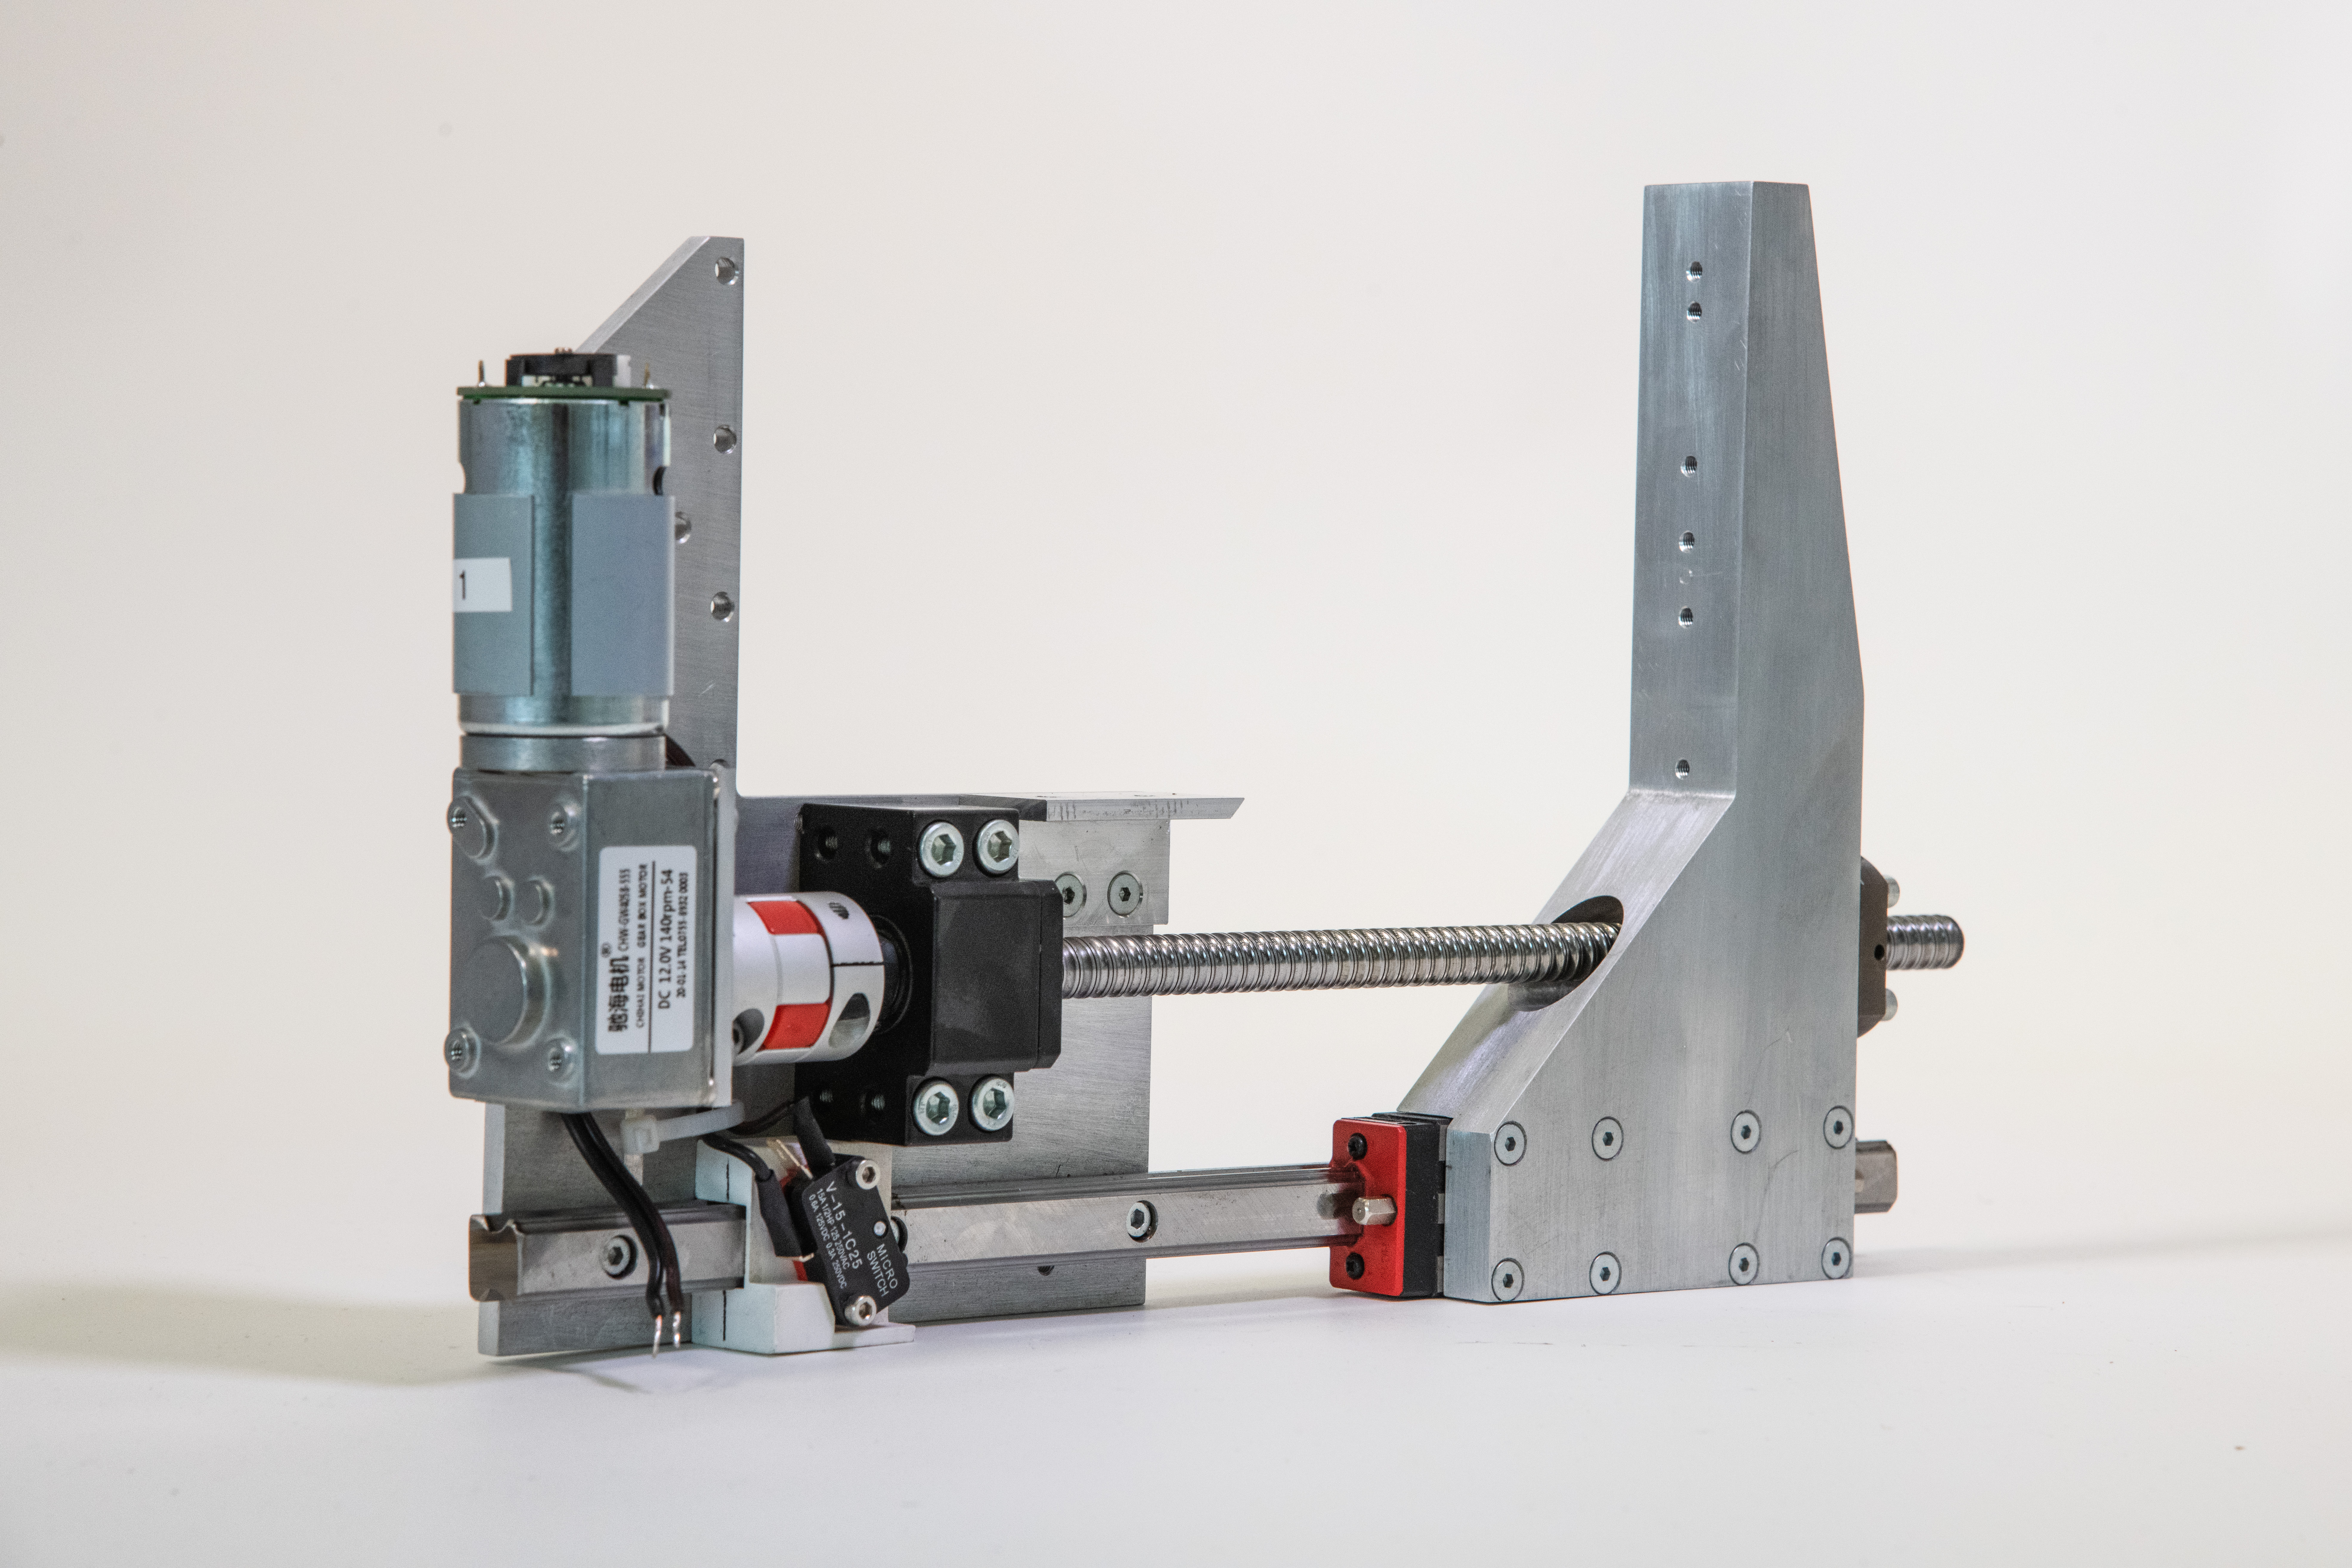
\includegraphics[width=15.92cm,height=13.44cm]{./images/image35.jpeg}
\end{figure}


\paragraph{Compute Object States}

During the assembly process, the state of the RFL Robot, Clamps, Grippers and Beams are changed from step to step. While the previous step has computed the location of all the objects attached to the kinematic chain, it is still necessary to keep track of the states of the other objects that are not attached to the chain.

\begin{figure}[H]
\includegraphics[width=15.92cm,height=5.19cm]{./images/image36.jpeg}
\end{figure}


The state of an object reflects what can be changed during the assembly process, therefore they belong to the extrinsic properties of the Models that represent them. The state includes more properties than just the pose of the object. For example, the Clamps and Grippers are kinematic and their collision geometry can change depending on their Joint Configuration (e.g. Gripper Finger position and Clamp Jaw position). The table below shows the state variables used for the Clamp Assembly Process.

\begin{table}[H]
\begin{adjustbox}{max width=\textwidth}
\begin{tabular}{p{3.7cm}p{5.0cm}p{7.22cm}}
\hline
\multicolumn{1}{|p{3.7cm}}{{\footnotesize \textbf{Object Type}}} & 
\multicolumn{1}{|p{5.0cm}}{{\footnotesize \textbf{Parameters}}} & 
\multicolumn{1}{|p{7.22cm}|}{{\footnotesize \textbf{Parameter Type}}} \\ 
\hline
\multicolumn{1}{|p{3.7cm}}{{\footnotesize RFL Robot}} & 
\multicolumn{1}{|p{5.0cm}}{\begin{itemize}
	\item {\footnotesize Joint Configuration} \newline
	\item {\footnotesize Target Frame}} & 
\multicolumn{1}{|p{7.22cm}|}{	\item {\footnotesize List of Joint Values} \newline
	\item {\footnotesize Rigid Transformation / Frame}} \\ 
\hline
\multicolumn{1}{|p{3.7cm}}{{\footnotesize Docking Adapter}} & 
\multicolumn{1}{|p{5.0cm}}{\begin{itemize}
	\item {\footnotesize Base Frame} \newline
	\item {\footnotesize Kinematic Attachment}} & 
\multicolumn{1}{|p{7.22cm}|}{	\item {\footnotesize Rigid Transformation / Frame} \newline
	\item {\footnotesize Parent Object, Rigid Transformation}} \\ 
\hline
\multicolumn{1}{|p{3.7cm}}{{\footnotesize Tools (Clamps and Grippers)}} & 
\multicolumn{1}{|p{5.0cm}}{	\item {\footnotesize Tool Frame} \newline
	\item {\footnotesize Joint Configuration} \newline
	\item {\footnotesize Kinematic Attachment}} & 
\multicolumn{1}{|p{7.22cm}|}{	\item {\footnotesize Rigid Transformation / Frame} \newline
	\item {\footnotesize List of Joint Values} \newline
	\item {\footnotesize Parent Object, Rigid Transformation}} \\ 
\hline
\multicolumn{1}{|p{3.7cm}}{{\footnotesize Beams}} & 
\multicolumn{1}{|p{5.0cm}}{	\item {\footnotesize Beam Frame} \newline
	\item {\footnotesize Kinematic Attachment}} & 
\multicolumn{1}{|p{7.22cm}|}{	\item {\footnotesize Rigid Transformation / Frame} \newline
	\item {\footnotesize Parent Object, Rigid Transformation}} \\ 
\hline
\multicolumn{1}{|p{3.7cm}}{{\footnotesize Environment Model}} & 
\multicolumn{1}{|p{5.0cm}}{	\item {\footnotesize Object Frame}\end{itemize}
} & 
\multicolumn{1}{|p{7.22cm}|}{	\item {\footnotesize Rigid Transformation / Frame}\end{itemize}
} \\ 
\hline
\end{tabular}
\end{adjustbox}
\caption{position and Clamp Jaw position). The table below shows the state variables used for the Clamp Assembly Process.Except for the Joint Configuration of the Robot, which is computed later by the MMMP solver, all the other states have to be computed in this step. The computation starts with a manually defined Initial State. This is a full description including the joint configuration of the robot. In the Clamp Assembly Process, the initial state has the following properties :}
\label{tab:position_and_clamp_jaw_position}\end{table}
\begin{itemize}
	\item Robot at parking position (gantry retracted up, arm folded in a compact way)

	\item All tools at their storage location

	\item Gripper fingers closed

	\item Clamp gripper closed, clamp jaw extended

	\item Beams positioned in a stack at beam storage location 

\end{itemize}
Each of the low-level tasks is now seen as a function that causes a state change. In practice, this is implemented as a function in the Task Classes where a Starting State can be passed into the function and the Ending State is produced by updating the relevant parameters.\includegraphics[width=15.92cm,height=2.08cm]{./images/image37.jpeg}

The table below shows all the task.UpdateState() function and what state parameters are being updated. For unaffected parameters, their states remain the same. Note that the Robot Motions (LM, FM and SM), require target parameters. These were computed in the previous step and are stored as parameters in the corresponding RobotMotion task objects. In addition, other targets such as TargetJawPosition for clamp jaw motion and TargetBeamFrame for operator to place beam were retrieved from the process parameters.

\begin{table}[H]
\begin{adjustbox}{max width=\textwidth}
\begin{tabular}{p{2.38cm}p{5.42cm}p{8.21cm}}
\hline
\multicolumn{1}{|p{2.38cm}}{{\footnotesize \textbf{Task Agents}}} & 
\multicolumn{1}{|p{5.42cm}}{{\footnotesize \textbf{Low Level Task}}} & 
\multicolumn{1}{|p{8.21cm}|}{{\footnotesize \textbf{AffectedParameters in UpdateState()}}} \\ 
\hline
\multicolumn{1}{|p{2.38cm}}{{\footnotesize RFL Robot}} & 
\multicolumn{1}{|p{5.42cm}}{{\footnotesize Linear Motion} \newline
{\footnotesize Free Motion}} & 
\multicolumn{1}{|p{8.21cm}|}{{\footnotesize Robot/TargetFrame $=$ \uline{TargetFrame}} \newline
{\footnotesize DockingAdapter/BaseFrame $=$  \uline{TargetFrame}} \newline
{\footnotesize Tool/ToolFrame $=$ \uline{TargetToolFrame }$\ast$} \newline
{\footnotesize Beam/BeamFrame $=$ \uline{TargetBeamFrame }$\ast$}} \\ 
\hline
\multicolumn{1}{|p{2.38cm}}{{\footnotesize RFL Robots and Clamp(s)}} & 
\multicolumn{1}{|p{5.42cm}}{{\footnotesize Clamp and Robot Sync Linear Motion}} & 
\multicolumn{1}{|p{8.21cm}|}{{\footnotesize Robot/TargetFrame $=$ \uline{TargetFrame}} \newline
{\footnotesize DockingAdapter/BaseFrame $=$  \uline{TargetFrame}} \newline
{\footnotesize Tool/ToolFrame $=$ \uline{TargetToolFrame}} \newline
{\footnotesize Beam/BeamFrame $=$ \uline{TargetBeamFrame}} \newline
{\footnotesize Clamp/JointConfig $=$ \uline{TargetJawPosition}}} \\ 
\hline
\multicolumn{1}{|p{2.38cm}}{\multirow{3}{*}{\parbox{2.38cm}{{\footnotesize Clamp}}}} & 
\multicolumn{1}{|p{5.42cm}}{{\footnotesize Clamp Jaw Motion}} & 
\multicolumn{1}{|p{8.21cm}|}{{\footnotesize Clamp/JointConfig/JawPosition $=$ \uline{TargetJawPosition}}} \\ 
\hhline{~--}
\multicolumn{1}{|p{2.38cm}}{} & 
\multicolumn{1}{|p{5.42cm}}{{\footnotesize Open Hanging Gripper}} & 
\multicolumn{1}{|p{8.21cm}|}{{\footnotesize Clamp/JointConfig/Gripper$=$ Open}} \\ 
\hhline{~--}
\multicolumn{1}{|p{2.38cm}}{} & 
\multicolumn{1}{|p{5.42cm}}{{\footnotesize Close Hanging Gripper}} & 
\multicolumn{1}{|p{8.21cm}|}{{\footnotesize Clamp/JointConfig/Gripper $=$ Close}} \\ 
\hline
\multicolumn{1}{|p{2.38cm}}{\multirow{2}{*}{\parbox{2.38cm}{{\footnotesize Parallel Gripper}}}} & 
\multicolumn{1}{|p{5.42cm}}{{\footnotesize Open Gripper (Beam)}} & 
\multicolumn{1}{|p{8.21cm}|}{{\footnotesize Gripper/JointConfig/Gripper $=$ Open} \newline
{\footnotesize Beam/KinematicAttachment $=$ None, None}} \\ 
\hhline{~--}
\multicolumn{1}{|p{2.38cm}}{} & 
\multicolumn{1}{|p{5.42cm}}{{\footnotesize Close Gripper (Beam, Grasp)}} & 
\multicolumn{1}{|p{8.21cm}|}{{\footnotesize Gripper/JointConfig/Gripper $=$ Close} \newline
{\footnotesize Beam/KinematicAttachment $=$ Gripper, Grasp}} \\ 
\hline
\multicolumn{1}{|p{2.38cm}}{\multirow{2}{*}{\parbox{2.38cm}{{\footnotesize Docking Adapter}}}} & 
\multicolumn{1}{|p{5.42cm}}{{\footnotesize Lock Tool (Tool)}} & 
\multicolumn{1}{|p{8.21cm}|}{{\footnotesize Tool/KinematicAttachment $=$ None, None}} \\ 
\hhline{~--}
\multicolumn{1}{|p{2.38cm}}{} & 
\multicolumn{1}{|p{5.42cm}}{{\footnotesize Unlock Tool (Tool)}} & 
\multicolumn{1}{|p{8.21cm}|}{{\footnotesize Tool/KinematicAttachment $=$ DockingAdapter, DockingAdapter.[Base]T[Child]}} \\ 
\hline
\multicolumn{1}{|p{2.38cm}}{{\footnotesize Operator}} & 
\multicolumn{1}{|p{5.42cm}}{{\footnotesize Place Beam in Robot Gripper}} & 
\multicolumn{1}{|p{8.21cm}|}{{\footnotesize Beam/BeamFrame $=$ \uline{TargetBeamFrame}}} \\ 
\hline
\end{tabular}
\end{adjustbox}
\end{table}
\vspace{4\baselineskip}
{\footnotesize $\ast$ Whether Tool and Beam Frame are updated depends on the kinematic chain configuration of that Robot Motion Task\par}

Because the task list is linear, the state update happens sequentially. The ending state of a task is used as the starting state input of the next task, this is continued until all the tasks are processed. I called the states in between \textbf{Intermediate States }and the last state as the \textbf{Final State, }or the \textbf{Goal State}.

\begin{figure}[H]
\includegraphics[width=8.01cm,height=8.99cm]{./images/image38.jpeg}
\end{figure}


When one of these states is used to update the extrinsic parameters of the object models, this is referred to as a \textbf{Scene \href{https://www.zotero.org/google-docs/?5iCzjM}{}(Moveit!, 2023)}. With the exception of the robot configuration, a scene is a complete description of all objects at a static moment. The diagram below shows a symbolic representation of the scene.

\begin{figure}[H]
\includegraphics[width=8.95cm,height=6.19cm]{./images/image39.jpeg}
\end{figure}


\vspace{1\baselineskip}
\paragraph{Process Visualization and Adjustment}

\begin{figure}[H]
\includegraphics[width=15.92cm,height=5.19cm]{./images/image40.jpeg}
\end{figure}


Up until this point, every parameter has been automatically computed from the initial Process Model and default values have been used for all the multiple-choice decisions. This step begins a cycle where the production engineer can visualize the assembly actions, identify problems, and make adjustments to the process parameters to correct them. Refer to \uline{6.3.5.3 Process Parameters} for the adjustable process parameters that are marked with Process Engineer (PE). Most of them are related to the gripper and the clamps. 

\subsection{Drawing Previews}

The following screen capture image shows how the process is visualised. A Rhino Command Interface was implemented to provide an interactive interface for the production engineer to step through the task list and visualise the scene at the end of each task. Extra controls are provided to jump to a specific beam or to skip through the non-robotic actions. The engineer is able to use all the 3D view control and rendering functions provided by the Rhino Viewport during this time.

Once a scene is selected, all the objects are drawn in the 3D modelling canvas based on the object models using their state parameters. The 3D models were initially implemented as mesh models because it is the default input format for motion planning. However, the implementation for visualisation was changed to using BRep Polysurfaces in Rhino because their solid boolean operations are easier to perform in Rhino. 

\begin{figure}[H]
\includegraphics[width=12.14cm,height=10.67cm]{./images/image41.jpeg}
\end{figure}


\subsection{User Interaction}

The interface also allows the engineer to make changes to the process parameters. The images below show the end of the ‘Clamp and Robot Sync Linear Motion’ for four different beams. The clamps (green). the gripper (dark blue) and the active beam (grey) can be seen. Notice that the robot configuration is not yet resolved (MP is next step) and therefore the robot cannot be displayed. However, because the robot’s spherical wrist is in a known position regardless of IK configuration, it can be represented with a sphere to check for possible collision.

{\small 1\includegraphics[width=7.64cm,height=4.3cm]{./images/image42.jpeg}2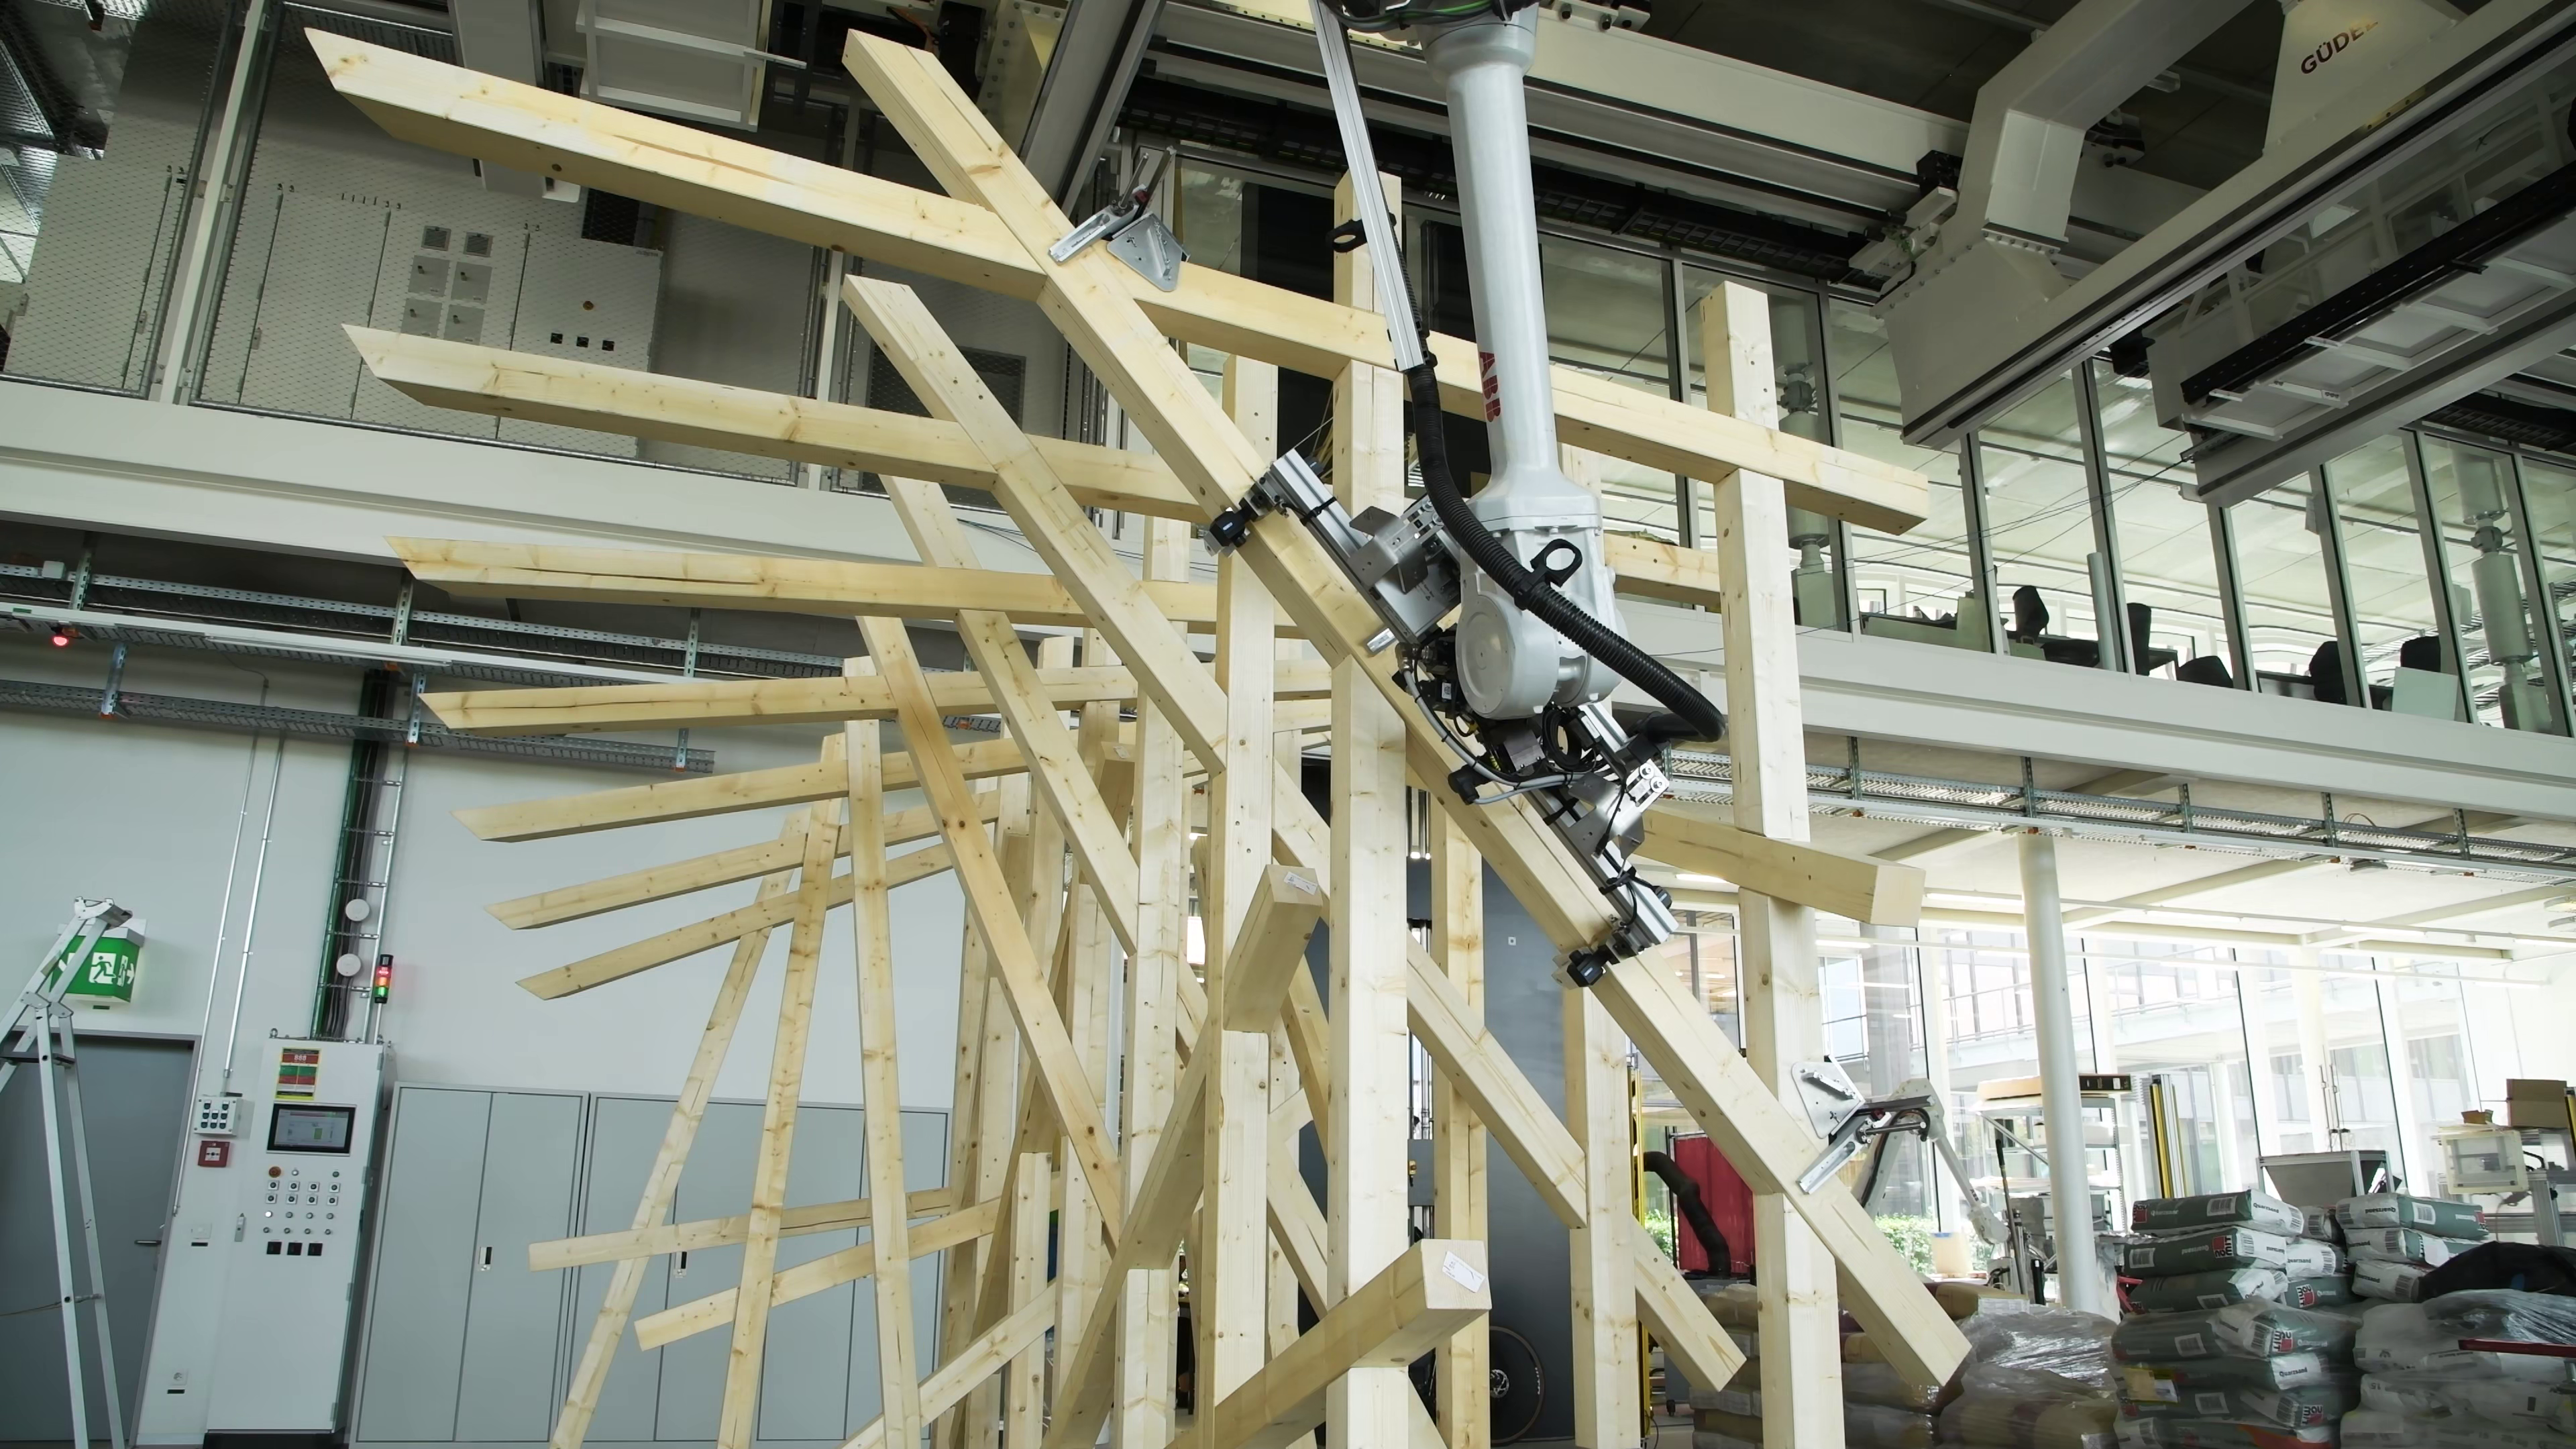
\includegraphics[width=7.64cm,height=4.32cm]{./images/image43.jpeg}}

{\small 3\includegraphics[width=7.64cm,height=4.32cm]{./images/image44.jpeg}4\includegraphics[width=7.64cm,height=4.32cm]{./images/image45.jpeg}}

The screen capture images below show the \textbf{visualisation of different steps }for one beam. 

\begin{itemize}
	\item Step 1 and 2 shows the clamps’ position before and after attaching the clamp to the PA structure. 

	\item Step 3 and 4 shows the gripper’s and beam’s positions before and after being moved into the clamp jaws. 

	\item Step 5 shows the position after the synchronised clamping.

	\item Step 6 shows the position after gripper release. 

	\item Step 7 and 8 shows the clamp position before and after being detached.

\end{itemize}
Notice that in this specific case, the position of the gripper before approach (3) and after retract (6) are not the same, therefore both positions need to be checked. In the case of collision, the objects would change colour as an indication.

{\footnotesize 1\includegraphics[width=7.64cm,height=4.3cm]{./images/image46.jpeg}2\includegraphics[width=7.64cm,height=4.32cm]{./images/image47.jpeg}}

{\footnotesize 3\includegraphics[width=7.64cm,height=4.32cm]{./images/image48.jpeg}4\includegraphics[width=7.64cm,height=4.32cm]{./images/image49.jpeg}}

{\footnotesize 5\includegraphics[width=7.64cm,height=4.32cm]{./images/image50.jpeg}6\includegraphics[width=7.64cm,height=4.32cm]{./images/image51.jpeg}}

{\footnotesize 7}\includegraphics[width=7.64cm,height=4.3cm]{./images/image52.jpeg}{\footnotesize 8}\includegraphics[width=7.64cm,height=4.32cm]{./images/image53.jpeg}

In the images below, there are no collisions in the clamped keyframe (left), but there are collisions in another keyframe (right). Therefore, the production engineer needs to go through each beam and each step to ensure they are all collision free. Otherwise the subsequent MP would fail to find a solution because the objects were already in collision. 

\begin{figure}[H]
\centering
\begin{subfigure}[b]{0.45\textwidth}
\centering
\includegraphics[width=\textwidth]{./images/image54.jpeg}
\end{subfigure}
\hfill
\begin{subfigure}[b]{0.45\textwidth}
\centering
\includegraphics[width=\textwidth]{./images/image55.jpeg}
\end{subfigure}
\end{figure}


In the next development round, an automatic collision check is implemented and the engineer only has to go through the problematic steps \textit{\textcolor[HTML]{B7B7B7}{(see \uline{7.3.21 Fast Design Validation with IK Check})}}.

Aside from collisions, the engineer can also make adjustments to avoid potentially difficult situations, such as beam grasp that are too close to other neighbours or the ground, or highly eccentric grasp that are prone to deflection. The ground platform can also be adjusted if necessary and updates the environment model. Once the engineer is happy with the Process Model, it can be passed on for motion planning. 

\paragraph{Multimodal Motion Planning (MMMP) Solver}

The MMMP solver implemented for this development round is responsible for planning the robotic motions in the tasks list. It has access to the Linear Motion planner and Free Motion Planner for planning the two different types of motion accordingly. Non-robotic motions in the task list are ignored.

\begin{figure}[H]
\includegraphics[width=15.92cm,height=5.19cm]{./images/image56.jpeg}
\end{figure}


The major role of the solver is to ensure \textbf{trajectory continuity} between neighbouring motions in the task list. In the initial development, this is ensured simply by planning the motions in a sequential way, such that the ending configuration of one motion can be used for the starting configuration of the next one. The diagram below shows how the ending configuration (C1) of a motion (M1) can be extracted from its planned trajectory. C1 can then be used for planning the next motion (M2).

\begin{figure}[H]
\includegraphics[width=15.92cm,height=8.47cm]{./images/image57.jpeg}
\end{figure}


In the case where MP failed, the planning routine was programmed to backtrack to the first motion of the failing beam (which is always a Free Motion) and restart the planning from there. The intention is that the highly stochastic FMP would result in a different ending configuration that is less likely to get stuck in the subsequent motion.

This downside of this sequential planning method was discovered not long after it was used. The algorithm often got stuck at one specific beam and cannot get past the beam. This created a design evaluation bottleneck when a full night (10h) of planning could only finish half of all the 40 beams, and the planning difficulty only increased towards the end because the partial structure became a large obstacle for the FMP.

This problem was addressed by separating the task list into smaller \textbf{task groups }organised by each beam, this created 40 groups for the 40 beams that could be planned in parallel, or skipped when being stuck. When the task lists had to be stitched back together, the Free Movement in the beginning of each beam can be replanned using the two neighbouring configurations to ensure their continuity. In conclusion, this discovery led to a generalizable approach of using \textbf{Free Motion as a ‘glue’} that can connect separately planned segments together \href{https://www.zotero.org/google-docs/?PykTOl}{(Lozano-Pérez $\&$ Kaelbling, 2014)}.

At a later stage of this Development Round, taught configuration was introduced for repetitive targets\textit{\textcolor[HTML]{B7B7B7}{ (see \uline{6.3.6 Taught configuration for Repetitive Targets})}}. This worsened the ‘stuck’ problem even within a Task Group. Another technique was subsequently developed to plan non-sequentially within a task group \textit{\textcolor[HTML]{B7B7B7}{(see \uline{6.3.7 Non-Sequential Planning Order})}}.

\paragraph{Short Discussion about Process Design}

The development of the planning process in this section is a process of discovery that has its own significance. 

Despite MP, TAMP and MMMP techniques have been demonstrated in many robotics research projects, applying them for timber construction, or architectural applications in general, require a significant adjustment to their parameters. Moreover, the integrated design and planning approach that is common in the architectural workflow has little precedence in the field of robotics where these algorithms were invented.

The development of High-Level Tasks, Low-Level Tasks, and the method of computing robot targets by geometrical relationship provided a unique solution for automatically parsing a design (i.e. the arrangement of beams and joints) into task and motion plans needed for autonomous execution. In addition, the discovery of process parameters that can have multiple options, formalised the workflow for how user input can be accommodated. It also opened the avenue for future work to automate these decisions using rule-based logic or searching techniques. This provided a roadmap for improving the process engineer’s role, from fixing collision problems, to designing the computational algorithms that can fix it automatically. 

Finally this development has shown that, the planning flowchart, the high level tasks, the low level tasks, the geometrical relationships between robot targets and the ACM are specific to the construction method (DiRT clamping in this case) and will require project specific customization. While the tasks performed by these algorithms are similar to the work of a construction planner, the skillset to design them is rather specialised. It is still uncertain as to who will design them.

\subsubsection{Taught configuration for Repetitive Targets}

Taught configuration \textit{\textcolor[HTML]{B7B7B7}{(introduced in Intro) }}was introduced as an additional parameter for defining a Robot Motion Task. This allows the production engineer to define a fixed robot configuration as targets for a specific motion \href{https://www.zotero.org/google-docs/?nTPVNG}{(Nof, 1999)}. It was used for repetitive targets such as tool storage pose and beam pickup pose to enhance the robotic accuracy for reaching them. This is because industrial robots have very good \textbf{repeatability }and can go back to the same absolute location, as long as the joint configurations remain the same. 

The photos below (left) shows the location where the tools are stored. A 3D-printed plastic pad (black) was used to position the tools in a repeatable position on the aluminium platform. The photo on the right shows a demonstration of \textbf{teaching }the robot configuration for picking up the tool. Similar process was used for the beam pickup configuration with the grippers.

\begin{figure}[H]
\centering
\begin{subfigure}[b]{0.45\textwidth}
\centering
\includegraphics[width=\textwidth]{./images/image58.jpeg}
\end{subfigure}
\hfill
\begin{subfigure}[b]{0.45\textwidth}
\centering
\includegraphics[width=\textwidth]{./images/image59.jpeg}
\end{subfigure}
\end{figure}


Taught configurations are typically acquired after the construction area is prepared and the storage stations are fixed. Considering a typical construction schedule (including this research project), it is unlikely that these configurations are available during the design and validation phase. In order to address this, an estimated configuration was used during the validation workflow \textit{\textcolor[HTML]{B7B7B7}{(see \uline{6.3.5 Process Design Workflow})}}. The configurations were updated after the construction area was prepared, and the configurations were taught. The affected motions were then replanned.

Initially, the taught configurations were planned using the concept of sequentially chained planning with target poses\textit{\textcolor[HTML]{B7B7B7}{ (compare this with 6.3.5.7 Multimodal Motion Planning (MMMP)) Solver}}. For example, in the diagram below,

\begin{enumerate}
	\item Motion M1 with no taught configuration would be planned normally and its resulting configuration (C1) becomes the starting config of the next Motion (M2). 

	\item Assuming that M2 has a Taught (a.k.a Fixed) Configuration (C2) as target, then the motion planner will plan between configuration C1 and C2. The only difference is that both starting and ending targets have a configuration instead of only one side.

	\item Motion M3 would use C2 as the starting configuration for planning, similar to M1.

\end{enumerate}
\begin{figure}[H]
\includegraphics[width=15.92cm,height=10.72cm]{./images/image60.jpeg}
\end{figure}


However, this sequential planning method did not work in practice, continue reading in the next section \textit{\textcolor[HTML]{B7B7B7}{(see \uline{6.3.7 Non-Sequential Planning Order})}}.

\subsubsection{Non-Sequential Planning Order}

After the introduction of the taught configuration in the task list, a new problem was discovered. The success rate of planning the task groups has dropped to zero - 0 success for each of the 40 beams (using 1800 seconds of maximum planning time).

Upon further investigation, the cause was identified to be the interaction between the taught configuration and the Linear Motion Planner as the problem occurs only if the taught configuration is used for Linear Motion target, but not Free Motion. The problem can be illustrated in the diagram below (space between boxes are reduced when compared to the diagram in the previous section). The diagram shows the sequential planning process for the PickToolFromStorage Task, note that this is only a portion of the Task Group for the whole beam. 

The red arrow denotes a fixed configuration input to the motion planner. It typically happens when the configuration is carried forward from the previous motion. The problem occurs when the Linear Motion M3 is planned, the Linear Motion Planner (LMP) receives fixed configuration for both start and end points. This over-constrained the LMP and the chance of successfully planning past this motion is almost zero.

\begin{figure}[H]
\includegraphics[width=15.92cm,height=12.88cm]{./images/image61.jpeg}
\end{figure}


\subsection{Solution and Follow-Up}

The following solution was considered but was not successful:

\begin{itemize}
	\item \textbf{Remove this Linear Motion }- it is not possible because of the narrow passage problem \textit{\textcolor[HTML]{B7B7B7}{(see \uline{5.5.3 Narrow Passage Problem})}}. 

	\item \textbf{Plan Sequentially Backwards} - the over constraint scenario will still be encountered.

\end{itemize}
The solution that successfully addressed the problem consist of three parts:

\begin{itemize}
	\item A \textbf{priority flag }was added to the Motion Task to signify that it should be planned first. 

	\item The process engineer can set this flag at the high-level task group template, and it would automatically appear in all motion tasks after Task Planning in the task list.

	\item The MMMP solver was modified to consider these flags and to plan the high priority task first. The diagram below depicts how the MMMP solver would evaluate the priority flag and plan with a custom sequence.

\end{itemize}
The details of this discovery and the planning method have already been published. For implementation details, refer to \href{https://www.zotero.org/google-docs/?W31fOF}{(Huang et al., 2021)}

\begin{figure}[H]
\includegraphics[width=15.92cm,height=9.35cm]{./images/image62.png}
\end{figure}


In summary, the departure from sequential planning order allowed the motions with more constraints (such as the Linear Motion next to a taught config) to be planned first. In this way, it was possible to avoid having both start and end config input for the LMP. The FMP, on the contrary, is able to handle the constraints and is planned the last. The following diagram depicts the same PickToolFromStorage Task. 

Using the new method, Motion M3 and M4 would be flagged by the Process Engineer to be planned first, each of them will have one fixed config (directly from the taught config). Then M2 will be planned next (because LM has a higher priority than FM), it will also have one fixed config. M1 and M5 will be planned last, and will likely have two fixed configurations due to their neighbours before and after them. The FMG will have a much higher chance of bridging between the two constraints. 

\begin{figure}[H]
\includegraphics[width=15.92cm,height=11.18cm]{./images/image63.jpeg}
\end{figure}


The following charts \href{https://www.zotero.org/google-docs/?LIhaZP}{(Huang et al., 2021)} shows the success rate and runtime for planning one task group (one beam) using the non-sequential (it is called nonlinear in the paper) versus sequential planning. Notice that the success rate for sequential planning is practically zero. 

\begin{figure}[H]
\includegraphics[width=15.92cm,height=4.73cm]{./images/image64.jpeg}
\end{figure}


\vspace{1\baselineskip}
\subsubsection{Standalone Process Execution Controller}

An improvement was made to upgrade the L3 Process Execution Controller that was based on Rhino Grasshopper \textit{\textcolor[HTML]{B7B7B7}{(see \uline{5.3.15 Process Execution Controller})}}. The new controller is written in Python 3 code and utilises Tkinter to create an interactive graphical user interface (GUI).

\begin{figure}[H]
\includegraphics[width=15.92cm,height=8.71cm]{./images/image65.jpeg}
\end{figure}


In addition to the previous capability of sending pre-planned motions to the L2 Robot Controller and L2 Clamp controller. It has the following new functionalities:

\begin{itemize}
	\item A table view of the sequential Task List organised by Beam and TaskGroup. 

	\item Provide a user interface for the operator to monitor the robot's state and execution progress.

	\item Provides synchronised motions between L2 Clamp Controller and L2 Robot Controller to execute ‘Clamp and Robot Sync Linear Motion’.

	\item Can send robot arm to the start or end state of action directly. (Useful for retrying an action)

	\item Can monitor sensor readings and robot status

	\item Log execution events and surveyed results

\end{itemize}
The tasks that were supported by the Execution Controller are listed in the task table in \uline{6.3.5.2 Expansion to Low Level Tasks}. Each task has a corresponding execution function that specifies how it should be executed. They were developed according to the protocols provided by the controllers that provided the execution capability, in this case, compas\_rrc (L2) and the L2 Clamp Controller. 

In theory each controller should provide a method to start a task, to query the state of the task, and to stop an ongoing task. However, the stopping function was not implemented in compas\_rrc until the next Dev Round. This means that it was still not possible to stop an ongoing motion or to keep the two controllers in sync during an error stop \textit{\textcolor[HTML]{B7B7B7}{(see \uline{5.6.9 Arm and Clamps Out-of-Sync after Error})}}.

\subsection{Operator Tasks}

There are two types of Operator Tasks in the process, OperatorLoadBeam and VisualInspection. When the execution controller encounters these tasks, a dialog will appear to show the operator the task instructions and the controller will wait for the operator to complete that task. The operator will need to click a button to confirm the task is finished before the next task is executed. 

\subsection{Execution Flow Control}

The controller maintains an execution pointer that points to a selected task in the list (the blue row in the image above). The controller has four states:

\begin{itemize}
	\item \textbf{Stopped }- The initial state, no task is being executed

	\item \textbf{Stepping }- This can be activated by the \textbf{Step Button}. The selected task will be executed immediately by the corresponding lower-level controllers. When the task is finished, the pointer will advance to point to the next task and the controller will go back to the Stopped state. This effectively executes only one task.

	\item \textbf{Running }- This can be activated by the \textbf{Run Button}. Similar to the stepping state, but after a task is finished, the controller will continue to execute the remaining tasks in the task list.

	\item \textbf{Error }- This state is entered automatically if the executing task has failed.

\end{itemize}
If the operator presses the \textbf{Stop Button}, the current task will be stopped immediately. The operator can also change from the Running state to the Step State at any time by using the \textbf{Step Button}. This effectively means the current task will be allowed to finish but the next one will not be started. 

\subsection{Challenges}

The main challenge faced in developing the controller is to synchronise emergency stop signals between different Level 2 controllers. As witnessed before, these stop signals could be thrown by the ABB Controller due to a variety of reasons (overload, collision, out of reach) and the clamp controller due to clamp stalling or loss of signal. However, the Level 2 to Level 3 communication channel that was based on compas\_rrc implementation only supported a sequential, first-in-first-execute approach. This prevented any unplanned signals (such as the emergency stop) from being communicated out of sequence.

\begin{table}[H]
\begin{adjustbox}{max width=\textwidth}
\begin{tabular}{p{7.04cm}p{1.67cm}p{7.17cm}}
\hline
\multicolumn{1}{|p{7.04cm}}{{\footnotesize \textbf{Level 3 Controller}}} & 
\multicolumn{1}{|p{1.67cm}}{{\footnotesize \textbf{Com}}} & 
\multicolumn{1}{|p{7.17cm}|}{{\footnotesize \textbf{Level 2 Controller (e.g. ABB Robot)}}} \\ 
\hline
\multicolumn{1}{|p{7.04cm}}{{\footnotesize Long Command 1 (e.g. Movement)}} & 
\multicolumn{1}{|p{1.67cm}}{\centering
{\footnotesize $\rightarrow$}} & 
\multicolumn{1}{|p{7.17cm}|}{{\footnotesize Move to execution queue}} \\ 
\hline
\multicolumn{1}{|p{7.04cm}}{{\footnotesize Long Command 2 (e.g. Movement)}} & 
\multicolumn{1}{|p{1.67cm}}{\centering
{\footnotesize $\rightarrow$}} & 
\multicolumn{1}{|p{7.17cm}|}{{\footnotesize Move to execution queue}} \\ 
\hline
\multicolumn{3}{|p{15.87cm}|}{{\footnotesize After Command 1 is completed}} \\ 
\hline
\multicolumn{1}{|p{7.04cm}}{{\footnotesize Update Command 1 status (e.g. Completed)}} & 
\multicolumn{1}{|p{1.67cm}}{\centering
{\footnotesize $\leftarrow$}} & 
\multicolumn{1}{|p{7.17cm}|}{{\footnotesize Status Update for Command 1}} \\ 
\hline
\multicolumn{3}{|p{15.87cm}|}{{\footnotesize Emergency Stop during the execution of Command 2}} \\ 
\hline
\multicolumn{1}{|p{7.04cm}}{} & 
\multicolumn{1}{|p{1.67cm}}{} & 
\multicolumn{1}{|p{7.17cm}|}{{\footnotesize Status Update is not initiated}} \\ 
\hline
\multicolumn{1}{|p{7.04cm}}{{\footnotesize Controller is not informed about the stop, e.g. the clamps are still running}} & 
\multicolumn{1}{|p{1.67cm}}{} & 
\multicolumn{1}{|p{7.17cm}|}{} \\ 
\hline
\end{tabular}
\end{adjustbox}
\end{table}
\vspace{4\baselineskip}
An workaround was implemented to solve this problem, providing some improvement. The approach is to send only a small amount of targets in a short horizon and upon detection of a stop condition, discontinue the commands. However, this approach still causes a small amount of out-of-sync distance after the stop signal. 

This problem was only truly resolved after this Dev Round when developers of compas\_rrc upgraded the system to support real-time commands being passed on a second channel. The second channel allows the Level 3 controller to query the system status of the Level 2 controllers and can be performed frequently enough to detect emergency signals.

\begin{table}[H]
\begin{adjustbox}{max width=\textwidth}
\begin{tabular}{p{7.04cm}p{1.67cm}p{7.17cm}}
\hline
\multicolumn{1}{|p{7.04cm}}{{\footnotesize \textbf{Level 3 Controller}}} & 
\multicolumn{1}{|p{1.67cm}}{{\footnotesize \textbf{Com}}} & 
\multicolumn{1}{|p{7.17cm}|}{{\footnotesize \textbf{Level 2 Controller (e.g. ABB Robot)}}} \\ 
\hline
\multicolumn{1}{|p{7.04cm}}{{\footnotesize Long Command 1 (e.g. Movement)}} & 
\multicolumn{1}{|p{1.67cm}}{\centering
{\footnotesize $\rightarrow$}} & 
\multicolumn{1}{|p{7.17cm}|}{{\footnotesize Move to execution queue}} \\ 
\hline
\multicolumn{1}{|p{7.04cm}}{{\footnotesize Long Command 2 (e.g. Movement)}} & 
\multicolumn{1}{|p{1.67cm}}{\centering
{\footnotesize $\rightarrow$}} & 
\multicolumn{1}{|p{7.17cm}|}{{\footnotesize Move to execution queue}} \\ 
\hline
\multicolumn{3}{|p{15.87cm}|}{{\footnotesize After Command 1 is completed}} \\ 
\hline
\multicolumn{1}{|p{7.04cm}}{{\footnotesize Update Command 1 status (e.g. Completed)}} & 
\multicolumn{1}{|p{1.67cm}}{\centering
{\footnotesize $\leftarrow$}} & 
\multicolumn{1}{|p{7.17cm}|}{{\footnotesize Status Update for Command 1}} \\ 
\hline
\multicolumn{3}{|p{15.87cm}|}{{\footnotesize Emergency Stop during the execution of Command 2}} \\ 
\hline
\multicolumn{1}{|p{7.04cm}}{} & 
\multicolumn{1}{|p{1.67cm}}{} & 
\multicolumn{1}{|p{7.17cm}|}{{\footnotesize Status Update is not initiated}} \\ 
\hline
\multicolumn{1}{|p{7.04cm}}{{\footnotesize Controller realised the ABB Robot Controller is not running using the \uline{second channel}}} & 
\multicolumn{1}{|p{1.67cm}}{} & 
\multicolumn{1}{|p{7.17cm}|}{} \\ 
\hline
\multicolumn{1}{|p{7.04cm}}{{\footnotesize Controller can propagate stop signal to other Level 2 controllers, e.g. stop the clamps}} & 
\multicolumn{1}{|p{1.67cm}}{} & 
\multicolumn{1}{|p{7.17cm}|}{} \\ 
\hline
\end{tabular}
\end{adjustbox}
\end{table}
\vspace{7\baselineskip}
\subsection{Lesson learnt from this development}

A generalizable lesson learnt regarding the communication protocol between Level 2 (L2) to Level 3 (L3) controllers is that the use of a sequential commanding structure is incompatible with the time-critical synchronisation process that involves multiple controllers. This is relevant not only to DiRT operation but also systems such as 3D printing where a robotic arm is moving an extruder and the extruder mechanism is controlled by a separate controller.

Despite the successful test using a two-channel approach, I propose the following modification for future communication protocol. In this proposal, only one communication channel is needed and is always treated as a real-time non-blocking channel. Similar to the current protocol, a command is initiated by the L3. However, it can have a number of possible states that can better represent the queue and error state caused by the L2 controller:

\begin{table}[H]
\begin{adjustbox}{max width=\textwidth}
\begin{tabular}{p{2.7cm}p{13.02cm}}
\hline
\multicolumn{1}{|p{2.7cm}}{{\footnotesize \textbf{States}}} & 
\multicolumn{1}{|p{13.02cm}|}{{\footnotesize \textbf{Meaning}}} \\ 
\hline
\multicolumn{1}{|p{2.7cm}}{{\footnotesize Queued}} & 
\multicolumn{1}{|p{13.02cm}|}{{\footnotesize Command is queued for execution because other commands are still running. }} \\ 
\hline
\multicolumn{1}{|p{2.7cm}}{{\footnotesize Queue Full Cancelled}} & 
\multicolumn{1}{|p{13.02cm}|}{{\footnotesize Command cannot be queued because the buffer is full.}} \\ 
\hline
\multicolumn{1}{|p{2.7cm}}{{\footnotesize Running}} & 
\multicolumn{1}{|p{13.02cm}|}{{\footnotesize Command is currently running}} \\ 
\hline
\multicolumn{1}{|p{2.7cm}}{{\footnotesize Paused}} & 
\multicolumn{1}{|p{13.02cm}|}{{\footnotesize Command is paused by the L3 controller after it has started running. It can be unpaused by the L3 controller and continue.\par}} \\ 
\hline
\multicolumn{1}{|p{2.7cm}}{{\footnotesize Completed}} & 
\multicolumn{1}{|p{13.02cm}|}{{\footnotesize Command is completed successfully}} \\ 
\hline
\multicolumn{1}{|p{2.7cm}}{{\footnotesize Error}} & 
\multicolumn{1}{|p{13.02cm}|}{{\footnotesize Command failed and cannot be continued. L2 Controller is likely to enter an error state and will not execute further until L3 cancels the error.\par}} \\ 
\hline
\multicolumn{1}{|p{2.7cm}}{{\footnotesize Cancelled}} & 
\multicolumn{1}{|p{13.02cm}|}{{\footnotesize The command is cancelled by the request of L3.}} \\ 
\hline
\end{tabular}
\end{adjustbox}
\end{table}
When the level 2 controller receives a command, it makes the decision whether the command is queued, or to start running immediately depending on the current buffering level within the controller. Level 3 can make a further request to change the command status to \textbf{Pause }or to \textbf{Cancel }the command. The following diagram listed out the change between the states. The label (L2 or L3) indicates which controller is able to initiate the change. 

For out-of-sequence commands, such as a status report request or a pause request, the Level 2 controller should directly execute the command upon reception and change its status to \textbf{Completed }immediately.

\begin{figure}[H]
\includegraphics[width=15.92cm,height=10.87cm]{./images/image66.jpeg}
\end{figure}


The following table illustrates the events during an emergency stop situation, how the Level 3 controller is informed, and how the error is cleared:

\begin{table}[H]
\begin{adjustbox}{max width=\textwidth}
\begin{tabular}{p{7.04cm}p{1.67cm}p{7.17cm}}
\hline
\multicolumn{1}{|p{7.04cm}}{{\footnotesize \textbf{Level 3 Controller}}} & 
\multicolumn{1}{|p{1.67cm}}{{\footnotesize \textbf{Com}}} & 
\multicolumn{1}{|p{7.17cm}|}{{\footnotesize \textbf{Level 2 Controller (e.g. ABB Robot)}}} \\ 
\hline
\multicolumn{1}{|p{7.04cm}}{{\footnotesize Long Command 1 (e.g. Movement)}} & 
\multicolumn{1}{|p{1.67cm}}{\centering
{\footnotesize $\rightarrow$}} & 
\multicolumn{1}{|p{7.17cm}|}{{\footnotesize Move to execution queue}} \\ 
\hline
\multicolumn{1}{|p{7.04cm}}{{\footnotesize Update Command 1 status (e.g. Running)}} & 
\multicolumn{1}{|p{1.67cm}}{\centering
{\footnotesize $\leftarrow$}} & 
\multicolumn{1}{|p{7.17cm}|}{{\footnotesize Non-blocking acknowledge / Status Update}} \\ 
\hline
\multicolumn{1}{|p{7.04cm}}{{\footnotesize Long Command 2 (e.g. Movement)}} & 
\multicolumn{1}{|p{1.67cm}}{\centering
{\footnotesize $\rightarrow$}} & 
\multicolumn{1}{|p{7.17cm}|}{{\footnotesize Move to execution queue}} \\ 
\hline
\multicolumn{1}{|p{7.04cm}}{{\footnotesize Update Command 2 status (e.g. Queued)}} & 
\multicolumn{1}{|p{1.67cm}}{\centering
{\footnotesize $\leftarrow$}} & 
\multicolumn{1}{|p{7.17cm}|}{{\footnotesize Non-blocking acknowledge / Status Update}} \\ 
\hline
\multicolumn{3}{|p{15.87cm}|}{{\footnotesize After Command 1 is completed}} \\ 
\hline
\multicolumn{1}{|p{7.04cm}}{{\footnotesize Update Command 1 status (e.g. Completed)}} & 
\multicolumn{1}{|p{1.67cm}}{\centering
{\footnotesize $\leftarrow$}} & 
\multicolumn{1}{|p{7.17cm}|}{{\footnotesize Status Update for Command 1}} \\ 
\hline
\multicolumn{1}{|p{7.04cm}}{{\footnotesize Update Command 2 status (e.g. Running)}} & 
\multicolumn{1}{|p{1.67cm}}{\centering
{\footnotesize $\leftarrow$}} & 
\multicolumn{1}{|p{7.17cm}|}{{\footnotesize Status Update for Command 2}} \\ 
\hline
\multicolumn{3}{|p{15.87cm}|}{{\footnotesize Emergency Stop during the execution of Command 2}} \\ 
\hline
\multicolumn{1}{|p{7.04cm}}{{\footnotesize Update Command 2 status (e.g. Error)}} & 
\multicolumn{1}{|p{1.67cm}}{\centering
{\footnotesize $\leftarrow$}} & 
\multicolumn{1}{|p{7.17cm}|}{{\footnotesize Status Update for Command 2}} \\ 
\hline
\multicolumn{1}{|p{7.04cm}}{{\footnotesize Controller can propagate stop signal to other Level 2 controllers, e.g. stop the clamps}} & 
\multicolumn{1}{|p{1.67cm}}{} & 
\multicolumn{1}{|p{7.17cm}|}{} \\ 
\hline
\multicolumn{3}{|p{15.87cm}|}{{\footnotesize Operator decides to clear the error}} \\ 
\hline
\multicolumn{1}{|p{7.04cm}}{{\footnotesize Cancel Command 2}} & 
\multicolumn{1}{|p{1.67cm}}{\centering
{\footnotesize $\rightarrow$}} & 
\multicolumn{1}{|p{7.17cm}|}{{\footnotesize Acknowledge / Remove command 2 from buffer}} \\ 
\hline
\end{tabular}
\end{adjustbox}
\end{table}
\vspace{3\baselineskip}
\subsection{Demonstration}

The demonstration structure is the same as the one used in the previous round. The timber beams were reused. The edges of lap joints that had less than 6mm chamfer were cut to 6mm, and those that were cut to 8mm still remained at 8mm \textit{\textcolor[HTML]{B7B7B7}{(see \uline{5.6.6 Clamping Joints with Chamfered Edges})}}. 

\subsubsection{Execution Plan}

The execution plan was similar to the previous construction except that no test fit was necessary and many of the manually performed tasks were performed robotically. After the construction of the ground platform, the planned tasks were executed sequentially as planned. The only planned operator actions were the loading of beams to the robot gripper. 

For the purpose of observation and debugging. A number of ``Operator Visual Inspection tasks'' were also added to the planning template for introducing a pause to the other automatic process. They were considered only necessary during the development process and are not integral to the DiRT Assembly Process. The inspection happens at the following movements:

\begin{itemize}
	\item Checking if the alignment was good at critical moments before proceeding.

\begin{itemize}
	\item Before docking approach

	\item Before moving a clamp to the attachment location on a joint.

\end{itemize}
	\item Checking if a clamp was stable before unlocking and undocking them.

	\item Checking if a placed beam is stable before releasing the gripper.

	\item Checking if a beam is stable after picking it up from the storage location.

\end{itemize}
\subsubsection{Construction Environment Setup}

The location of the new ground platform \textit{\textcolor[HTML]{B7B7B7}{(see \uline{6.3.1 Ground Platform Redesign})}} was located in a more central position under the robotic gantry in the robotic lab. This reduced the difficulty of the motion planning because there was more room on the sides for the robot to manipulate the long beams. The image below shows the controller’s console in relation to the ground platform.

\begin{figure}[H]
\includegraphics[width=15.92cm,height=10.62cm]{./images/image67.jpeg}
\end{figure}


The image below shows the collision model used for the environment. The taught positions of the tools (red) can also be seen \textit{\textcolor[HTML]{B7B7B7}{(see \uline{6.3.6 Taught configuration for Repetitive Targets})}}.

\begin{figure}[H]
\includegraphics[width=15.92cm,height=7.97cm]{./images/image68.jpeg}
\end{figure}


The photo below shows the four screwdrivers (CL3 and CL3M) and the short gripper (PG500) placed in their storage location. The reused timber beams of the BusStop Pavilion can be seen in the background, sorted, and ready for assembly. The holes used to adjust column height in the last test can be seen at some column ends. These holes were not used in this round because the columns will sit flush with the aluminium platform.

\begin{figure}[H]
\includegraphics[width=15.92cm,height=8.96cm]{./images/image69.jpeg}
\end{figure}


\subsubsection{Scaffolding and Screw Test}

After the previous round, it was clear that the new robotic operations would not be possible if the PA structure had a large deformation. Therefore, aluminium bars were added during construction by manually clamping them to the structure. They simulate a scenario where the stationary-side structure is properly supported and does not deform substantially. This allowed the study of the robot-side inaccuracy separate from the stationary-side.

\begin{figure}[H]
\includegraphics[width=15.92cm,height=8.96cm]{./images/image70.jpeg}
\end{figure}


Wood screws were also added to the lap joint to prevent loose joints from opening up after they were assembled \textit{\textcolor[HTML]{B7B7B7}{(see \uline{5.6.15 Joints Loosening after Assembly})}}. 

\subsection{Lessons Learnt}

\subsubsection{Successful Validation}

\paragraph{Automatic Clamp Placement}

The automatic placement and retrieval of clamps was found to be possible, thereby validating one of the core principles of the Distributed Robotic Tools (DiRT) system. 

However, the process is not capable of full autonomy because of alignment problems and the lack of sensors that can detect the misalignment \textit{\textcolor[HTML]{B7B7B7}{(see 6.5.2 Beam Placement Misalignment and 6.5.3 Docking Adapter Misalignment)}}. This required the operator to constantly monitor the system by physically walking into the construction area. Not only that it is dangerous but also not very effective because many of the alignment locations are far from the ground. 

The photo below shows the robot having picked-up a clamp from the structure. A jerry rigged camera (pink) can be seen installed on the flange to help with docking alignment \textit{\textcolor[HTML]{B7B7B7}{(see \uline{6.5.5 Docking Adapter Alignment with Camera})}}. 

\begin{figure}[H]
\includegraphics[width=15.92cm,height=7.62cm]{./images/image71.png}
\end{figure}


\paragraph{Stability by Scaffolding}

The manual addition of scaffolding to support the columns was found to be helpful in stiffening the structure, indicating that this could be a viable strategy for future construction process. The photo below shows the scaffolding bars added to stabilise the structure. The location of the bars were determined on-the-spot by the operator by observing how the structure would lean or deform. This intuitive estimation was found to be possible. However, the associated problem with these added elements is that the robot can collide with it \textit{\textcolor[HTML]{B7B7B7}{(see \uline{6.5.6 Robot Collision with Scaffolding})}}.

\begin{figure}[H]
\includegraphics[width=15.92cm,height=10.62cm]{./images/image72.jpeg}
\end{figure}


\paragraph{Screws Preventing Joints Opening Up}

A small wood screw (5 x 80mm) was added manually to some of the lap joints to prevent them from opening up. 

After the clamping operation of a beam and during the release of the clamp, the tightness of the lap joint was assessed by the operator. A manual push was used to determine if the joints needed to be fixed. If so, a battery-powered screwdriver was used to insert a screw into the lap joint, penetrating the two beams. No pre-drilled holes were used because of the small screw size. 

Despite the small size of the screw, it was found to be sufficient in holding the joint in place, preventing them from opening up. They also appeared to have helped stiffen the structure. However, this effect was not conclusive.

Theoretically, this screw is not bearing the structural load of the structure, but only to prevent joints from accidentally opening up. This discovery provided useful information for later development of a screwdriver for closing joints in the next Dev Round (see 7.1 Goal). 

\paragraph{Debugging with the Process Execution Controller}

The process execution controller \textit{\textcolor[HTML]{B7B7B7}{(see \uline{6.3.8 Standalone Process Execution Controller})}} was found to be very helpful during the execution of the planned tasks. 

\begin{itemize}
	\item \textbf{Rewind and try again - }Using the task list in the table view, it is easy to select an earlier state to rewind the robot and tools back to an earlier state for debugging purposes.

	\item \textbf{Reprogramme the execution behaviour} - Because the \textit{execute() }function for each type of task is only binded when the L3 controller loads the planned tasks and motion. The execution behaviour can be changed easily during the debugging phase by modifying the execution code and reloading the planned motions. For example, the \textit{Lock Tool }task by the docking adapter was modified this way to include checking new sensors \textit{\textcolor[HTML]{B7B7B7}{(see \uline{7.3.9 Docking Adapter Lock Sensor})}}.

	\item \textbf{Table view provided a good overview - }The table view of tasks provided a good overview of what is about to be executed, This increased the confidence of the operator to not worry about incorrect programming causing dangerous execution.

	\item \textbf{Logging - }The data that can be logged with this system was found to be very helpful in debugging. The almost-real-time commands and replies from various controllers would otherwise be impossible to read from a console.

\end{itemize}
\subsubsection{Beam Placement Misalignment}

Despite the inclusion of temporary scaffolding during construction, which minimised the deformation of the partial structure, the beam alignment at its target position is still very poor.

\begin{itemize}
	\item For beams that are aligning to an already-assembled beam, the misalignment is too bad to be clamped successfully. 

\begin{itemize}
	\item On many occasions, I manually jogged the robot to try to align the joints visually. The deviation often requires 10 to 20mm of offset on the linear gantry and 2 to 4 degrees on the last joint of the robotic arm to be corrected. No pattern was observed between the offset amount.

	\item I have to perform this function so often that I added an `OperatorAddVisualOffset` Movement in the list of tasks and created a function for applying the offset to subsequent assembly and gripper retract movement. 

\end{itemize}
	\item For beams that are placed on the ground platform, the final target is somewhat consistently lower than the point where the beam touches the platform. 

\begin{itemize}
	\item This usually pushes the beam to slip within the gripper fingers but can sometimes cause an overload error on the robot controller.

	\item The position where the beam touches the platform is occasionally deviating on the horizontal plane. This was conveniently measurable with a tape measure because the vertical elements are arranged in a grid.

\end{itemize}
\end{itemize}
\subsection{Intermediate Solution}

Because of poor alignment, a temporary solution was added to allow the operator to offset the joint values such that the assembly process can continue. The operator was able to make adjustment for all nine axis and make small movements using an trial and error approach. The following graph plots the offsets that was applied to the robot for successfully aligning and docking with the tool changer when retrieving a clamp from the structure.

{\footnotesize \begin{figure}[H]
\includegraphics[width=10.0cm,height=8.1cm]{./images/image73.png}
\end{figure}
}

{\footnotesize Number of measured data points $=$ 29 \\ Mean Value (after discarding top and bottom 5$\%$ outlier) $=$ 9.1}

Although the data shows the distribution of the deviation, it is not possible to draw conclusion whether the inaccuracy comes from the robot-side or the stationary-side. It is most likely a combination of thetwo because the clamps also visibly move during the clamping movement. 

\subsection{Possible Cause}

Another investigation was conducted for the placement of beams when the misalignment was bad. Two different types of observations were made, to compare real world position and the position in the CAD model. In both cases, gripper-to-beam positions were first checked to ensure it is grasped correctly.

\begin{itemize}
	\item \textbf{Alignment to the ground platform} - Since the platform is measured with iGPS, its position in the CAD environment is highly accurate. The beam was sent to a known target above the platform, and its deviation is measured against it. In some cases, the error in the vertical direction is more than 10mm from the model in the CAD software. 

	\item \textbf{Alignment to other joints on the PA structure} - Since the PA structure sits accurately on the ground platform, and is supported by scaffolding, the location of the joints are reasonably accurate. However, misalignments between mating joints can also exceed 10mm. 

\end{itemize}
Because of these two observations I concluded that the source of error on the robot-side is so significant that no matter how stable the PA structure is, it is still beyond what the chamfered edges can correct. 

The following list explored the possible source of error on the robot-side in the kinematic chain, starting from the gantry, ending at the timber.

\begin{itemize}
	\item \textbf{Robotic platform}

\begin{itemize}
	\item Inaccuracy due to the mechanical system

	\item Inaccuracy due to the IK / FK conversion

\end{itemize}
	\item \textbf{Docking adapter}

\begin{itemize}
	\item The docking adapter is a commercially available and reliable component, the docking accuracy is published by Schunk to be 0.015mm. Although no data is available for orientation error, it is not likely to be the major factor.

\end{itemize}
\end{itemize}
\subsection{PG Gripper}

\begin{itemize}
\begin{itemize}
	\item The gripper is inspected for CAD-to-reality error. The build was found to be fairly accurate, likely within 0.5mm deviation. This source of error cannot be the major factor.

\end{itemize}
\end{itemize}
\subsection{Slip between PG Gripper and Beam during beam transfer}

\begin{itemize}
\begin{itemize}
	\item This is ruled out because the grasp pose is confirmed to be accurate before the measurement.

\end{itemize}
\end{itemize}
\subsection{Beam and Joint Geometry}

\begin{itemize}
\begin{itemize}
	\item This is ruled out after measurement. The deviations of the beam between joint positions are all within 1mm. Furthermore, the structure is known to fit together.

\end{itemize}
\end{itemize}
\subsection{Possible Solution and Follow-Up}

The only possible explanation of the large deviation (in the range of >10mm) is the error from the robotic platform. This led to a separate investigation in the next Dev Round (link) to determine the severity of the robot’s inaccuracy.

\subsubsection{Docking Adapter Misalignment}

Similar to the problem mentioned in the previous section. The misalignment between the robot-side and the tool-side of the docking adapter can also be severe enough that the conical part of the robot-side adapter cannot be inserted into the tool-side. This happened in two scenarios:

\begin{itemize}
	\item When trying to pick up used clamps from the PA structure (PickClampFromStructure). There is a less than 10$\%$ success rate.

	\item When picking up a clamp from storage (PickClampFromStorage), the alignment is very good and is 100$\%$ successful. The difference between the two cases is that the storage position is a taught configuration.

\end{itemize}
In these cases, either I manually jogged the robot to alignment, or pushed the PA Structure such that the adapter aligns. For the jogged cases, the approach is similar to the previous section, the following plot shows the offset distance:

{\footnotesize \begin{figure}[H]
\includegraphics[width=10.0cm,height=8.1cm]{./images/image74.png}
\end{figure}
}

{\footnotesize Number of measured data points $=$ 54 \\ Mean Value (after discarding top and bottom 5$\%$ outlier) $=$ 10.7mm}

\textbf{\uline{Possible Cause}}

The cause is similar to those mentioned in 6.5.1 Beam Target Misalignment. However, the fact that the clamp is hanging from the PA structure is likely to have more error. Unfortunately this was difficult to quantify. 

Note that the maximum permissible XY axis offset for the Schunk Tool Changer to successfully lock is 2mm, which is significantly smaller tolerance than the timber joints. This may explain the very low success rate

In the case of PickClampFromStorage, the use of taught configuration, resulting in 100$\%$ success rate confirms that the robot is very repeatable. 

\textbf{\uline{Possible Solution and Follow-Up}}

\begin{itemize}
	\item \textbf{Taught configuration} is confirmed to be very accurate. They are used for all repeatable positions in future demonstrations, such as tool storage positions and material pickup positions.

	\item \textbf{Redesign the docking adapter} to accept more deviation.

\begin{itemize}
	\item Not pursued because of budget limitations.

\end{itemize}
	\item \textbf{Active Correction by camera marker guidance} - A camera mounted on the robot-side, looking at a fiducial marker mounted on the tool-side to guide the robot into alignment.

\begin{itemize}
	\item Developed and tested successfully in Dev Round 4 (link)

\end{itemize}
	\item  \textbf{Active Correction by docking probe} - A two-axis joystick like probe can be used to guide the robot into alignment.

\begin{itemize}
	\item Not pursued in favour of the non-contact alignment method. The camera method can directly acquire the deviation in 6DOF, which is more capable than a mechanical solution.

\end{itemize}
\end{itemize}
\subsubsection{Docking Adapter Fail to Lock}

In some occasions, after the docking adapter is inserted within each other, and the pneumatic lock on the robot-side is activated, the docking adapter would fail to lock. This sets off a series of cascading events that, if not stopped, could result in damage:

\begin{enumerate}
	\item The failure to lock could not be detected automatically because the lock sensor (which is already integrated to the roboti-side) was not connected.

	\item The execution controller was not programmed to acquire a confirmation signal but simply assume the lock was successful after 4s. Therefore the execution pointer is moved to the next movement.

	\item The next movement is to release the clamp, this is performed by actuating the pneumatic clamp gripper through the feed-through on the docking adapter.

	\item Because the lock was not successful, the feed-through would leak causing a loud noise. Typically this would alert me to stop the system and fix the problem.

	\item If the system is not stopped in time, the execution controller would continue to move the execution pointer to the next move because the gripper actuator also lacks a sensor to detect its failure.

	\item The next two movements are the robotic arm detaching the clamp with linear movements. Since the clamp is not properly locked to the robotic arm and that the gripper is not released, the robotic arm moving away from the clamp can cause it to bend around the attachment location and result in a fall. 

\end{enumerate}
Fortunately, this problem has always been detected and stopped at step 4. I can then fix the problem by 

\begin{itemize}
	\item \textbf{Rewinding the execution state }to before the activation of the lock, give the clamp a push while attempting to activate the lock again. In most of the cases, the shaking solves the problem. However, when this doesn’t work,

	\item \textbf{I can manually jog the robot} in small linear or orientation increments before trying the lock again. It is relatively time consuming when manual jog is needed.

\end{itemize}
\textbf{\uline{Possible Cause}}

\begin{itemize}
	\item \textbf{Robotic arm or the clamp attachment being too stiff} - Even though the docking adapter is inserted, the locking action requires at least one of the two sides to be flexible enough to be pulled together. Even though the misalignment may be small, the stiffness on both sides prevents the lock from closing the gap.

\begin{itemize}
	\item Note that automatic tool changers, like this Schunk SWA 040, are designed for tool change at a storage location. The tool-side is often not held down by a stiff attachment.

\end{itemize}
	\item \textbf{Alignment deviation too large }- Even though the adapter is inserted into each other, the deviation can still be larger than the allowable tolerance.

\begin{itemize}
	\item Docking adapter is not oriented accurately.

	\item Docking adapter is not inserted deep enough.

\end{itemize}
\end{itemize}
\textbf{\uline{Possible Solution and Follow-Up}}

\begin{itemize}
	\item \textbf{Redesign the docking adapter} to acquire lock even under deviation. And the docking accuracy is regained after one of the sides is no longer stiff.

\begin{itemize}
	\item Not pursued because of budget limitations.

\end{itemize}
	\item \textbf{Enable compliance control on robotic arm }- reduce stiffness of the robotic arm side after insertion is successful

\begin{itemize}
	\item Tested with success (link) but only in combination with the camera correction method.

\end{itemize}
	\item \textbf{Active Correction by camera marker guidance} - Same as mentioned before \textit{\textcolor[HTML]{B7B7B7}{(see \uline{6.5.3 Docking Adapter Misalignment})}}

\begin{itemize}
	\item Developed and tested successfully in Dev Round 4 (link)

\end{itemize}
	\item \textbf{Shake the robot-side automatically} - The robot can be programmed to perform a small shaking movement similar to the one performed by hand.

\begin{itemize}
	\item Developed and tested successfully in Dev Round 4 (link)

\end{itemize}
\end{itemize}
\subsubsection{Docking Adapter Alignment with Camera}

In an attempt to understand if the docking adapter alignment can be solved by a camera solution. I attached a small WiFi camera (based on Raspberry Pi CAM) on the tool-side of the docking adapter, and attached a small calibration target pattern printed on paper and glued to a mounting bracket.

\begin{figure}[H]
\includegraphics[width=15.92cm,height=8.96cm]{./images/image75.jpeg}
\end{figure}


\begin{figure}[H]
\centering
\begin{subfigure}[b]{0.45\textwidth}
\centering
\includegraphics[width=\textwidth]{./images/image76.jpeg}
\end{subfigure}
\hfill
\begin{subfigure}[b]{0.45\textwidth}
\centering
\includegraphics[width=\textwidth]{./images/image77.jpeg}
\end{subfigure}
\end{figure}


(captions captions)

An alignment routine was added to the Process Execution Controller to involve the operator for aligning the docking adapter. A video feed with digitally overlaid blue and red marks was shown to the operator and the operator can type in misalignments values. The XY misalignment can be read from the red mark position over the target and the Z misalignment (distance to target) can be guessed using the position of the blue marks. The robot is then instructed to move to the offsetted position and the observation is repeated until all marks are aligned as best as possible. 

Due to the activation of only three Cartesian axes, the correction can only compensate for position but not orientation error. 

\subsection{Observation}

This method was tested 59 times.  It often takes a few attempts for the operator to align all the marks. The resulting success rate for the tool changer to insert the conical part into the tool-side is above 90$\%$. However, even though the insertion can be successful, the problem of failing to lock was still present. The following plot shows the offset that was applied to successfully dock with the docking adapter.

\textbf{\uline{\begin{figure}[H]
\includegraphics[width=11.43cm,height=8.94cm]{./images/image78.png}
\end{figure}
}}

{\footnotesize Number of measured data points $=$ 59 \\ Mean deviation value (after discarding top and bottom 5$\%$ outlier) $=$ 10.04mm\par}

\textbf{\uline{Possible Solution and Follow-Up}}

This experiment indicated that the visual docking method is a promising approach. Leading to the development of a fully automatic camera marker correction mechanism in the next Dev Round (link). 

After this positional correction and successful insertion, the docking adapter is still suffering from failure to lock. This indicated that the locking problem is likely the result of orientation error and overly stiff docking pair. Refer to Section\uline{ 6.5.4 Docking Adapter Fail to Lock} for the follow-up actions taken.

\subsubsection{Robot Collision with Scaffolding}

Due to the unplanned use of scaffolding to support the unstable structure. The pre-planned robotic motion caused collision of the moving objects with the scaffolding bar and clamps. 

{\large \textbf{\begin{figure}[H]
\includegraphics[width=15.92cm,height=8.96cm]{./images/image79.png}
\end{figure}
}}

\begin{figure}[H]
\centering
\begin{subfigure}[b]{0.45\textwidth}
\centering
\includegraphics[width=\textwidth]{./images/image80.png}
\end{subfigure}
\hfill
\begin{subfigure}[b]{0.45\textwidth}
\centering
\includegraphics[width=\textwidth]{./images/image81.png}
\end{subfigure}
\end{figure}


Collisions also happened with the documentation camera on a tripod. However, that camera is unrelated to the construction process.

\textbf{\uline{Possible Solution and Follow-Up}}

\begin{itemize}
	\item \textbf{Include scaffolding in motion planning }- in Dev Round 5, the use of scaffolding is a planned act. The location and geometry of the scaffolding bars can therefore be included as collision geometry during motion planning. \textit{\textcolor[HTML]{B7B7B7}{(see \uline{8.3.2 Scaffolding Support During Assembly)}}}.

	\item \textbf{Sensing collision geometry around robot }- If a dynamic point cloud scanner were to be used for scanning the area surrounding the robot during operation, the robot can potentially navigate around the newfound obstacle and would not be limited to the planned collision geometry. 

\begin{itemize}
	\item Existing research literature in autonomous robotics have developed many different techniques for sensing and replanning. \href{https://www.zotero.org/google-docs/?7DB2Nw}{(Elbanhawi $\&$ Simic, 2014)} However, due to the lack of expertise in these fields, the development was not pursued.

\end{itemize}
	\item \textbf{Do not use scaffolding }- in Dev Round 4, deformation-aware design principles and error correction method was developed \textit{\textcolor[HTML]{B7B7B7}{(see \uline{7.1.1 Deformation-Awareness and Error Correction by Triangulation})}}. The demonstrator can be designed to be stable and with limited deformation for all the incomplete states in the entire assembly process. This eliminated the need for any scaffolding during assembly. 

\end{itemize}
\subsubsection{Redundant Clamp Detach Attach Actions}

The task planning method using a flowchart was found to produce a number of redundant tasks regarding tool changes. This is because of the cyclic nature of the flowchart that considered only the tasks necessary for one beam. 

\textbf{\uline{Cause}}

In order to illustrate the problem, consider the task list below for two beams (b1 and b2). Each of them was clamped using the same clamps (c1, c2). They would have an almost identical task list such as the following:

\begin{enumerate}
	\item {\footnotesize Tasks for Beam (b1) }

\begin{enumerate}
	\item {\footnotesize PickClampFromStorage (c1)}

	\item {\footnotesize PlaceClampToStructure (c1)}

	\item {\footnotesize PickClampFromStorage (c2)}

	\item {\footnotesize PlaceClampToStructure (c2)}

	\item {\footnotesize PickGripperFromStorage (g1)}

	\item {\footnotesize PickBeamFromStorage (b1)}

	\item {\footnotesize PlaceBeamInClamp (b1, g1, [c1])}

	\item {\footnotesize AssembleBeamWithClamps (b1, g1, [c1])}

	\item {\footnotesize PlaceGripperToStorage (g1)}

	\item {\footnotesize PickClampFromStructure (c2)}

	\item {\footnotesize PlaceClampToStorage (c2)}

	\item {\footnotesize PickClampFromStructure (c1)}

	\item {\footnotesize PlaceClampToStorage (c1)}

\end{enumerate}
	\item {\footnotesize Tasks for Beam (b2) }

\begin{enumerate}
	\item {\footnotesize PickClampFromStorage (c1)}

	\item {\footnotesize PlaceClampToStructure (c1)}

	\item {\footnotesize PickClampFromStorage (c2)}

	\item {\footnotesize PlaceClampToStructure (c2)}

	\item {\footnotesize PickGripperFromStorage (g1)}

	\item {\footnotesize PickBeamFromStorage (b2)}

	\item {\footnotesize PlaceBeamInClamp (b2, g1, [c1])}

	\item {\footnotesize AssembleBeamWithClamps (b2, g1, [c1])}

	\item {\footnotesize PlaceGripperToStorage (g1)}

	\item {\footnotesize PickClampFromStructure (c2)}

	\item {\footnotesize PlaceClampToStorage (c2)}

	\item {\footnotesize PickClampFromStructure (c1)}

	\item {\footnotesize PlaceClampToStorage (c1)}

\end{enumerate}
\end{enumerate}
Notice that at the end of the first beam and the beginning of the next one, the robot will PickClampFromStructure (c1), PlaceClampToStorage (c1), PickClampFromStorage (c1), and finally PlaceClampToStructure (c1). The PlaceClampToStorage (c1) and PickClampFromStorage (c1) are redundant. Cancelling out these two actions would allow the clamp to go directly from one area of the structure to another area directly.

Conceptually, this is a simple elimination step. However, because the flow chart method is iterating based on one cycle per beam, it is difficult to reason about when to retrieve the clamps or not based on the situation in the previous or next beams. Furthermore, if a clamp is left on the structure, to be retrieved at a later time, there is no guarantee that the clamp can still be accessible. For example, the access could have been blocked by the addition of elements. 

\textbf{\uline{Possible Solution and Follow-Up}}

This problem is a classical reason for using automatic task planning that is developed by the robotics community \href{https://www.zotero.org/google-docs/?DFFCVl}{(Ghallab et al., 2016)}. The idea is to create rules for the computer to automatically search for an assembly task list. During a search, the computer can plan out when and how the clamps are moved, and whether it is necessary to place the clamp back to storage. 

The implementation of automated task planning is developed and tested in the next Dev Round \textit{\textcolor[HTML]{B7B7B7}{(see \uline{8.2.2 TAMP with PDDLStream} and \uline{8.3.5 Specifying Actions and Goals for TAMP with PDDLStream})}}. The results showed that a large amount of clamp transfer does not need to go back to storage \textit{\textcolor[HTML]{B7B7B7}{(see \uline{8.5.2.3 Optimised Clamp Transfer Tasks})}}.

\subsubsection{Difficulty in attaching beam to platform}

The ground platform in this round was designed for accurate measurement of robotic precision. However, during construction, attaching the columns to the flat surface of the aluminium profile proved challenging (see photo below, left). In many instances, a significant number of aluminium profiles were needed to provide a clamping surface between the column and the platform (see photo below, right). This is slow to erect, and the connection is not very stiff.

\begin{figure}[H]
\centering
\begin{subfigure}[b]{0.45\textwidth}
\centering
\includegraphics[width=\textwidth]{./images/image82.jpeg}
\end{subfigure}
\hfill
\begin{subfigure}[b]{0.45\textwidth}
\centering
\includegraphics[width=\textwidth]{./images/image83.jpeg}
\end{subfigure}
\end{figure}


\textbf{\uline{Possible Solution and Follow-Up}}

The experience from constructing the BusStop pavilion indicated that it would be beneficial if the first few elements could be anchored to the platform with more than one connection. In order to achieve this, the design of the structure has to allow for this. This concept was tested when designing the next two demonstrators and was found to improve the stability substantially.

\subsubsection{Difficult to Plan Targets}

The chart below  \href{https://www.zotero.org/google-docs/?U91Ddz}{(Huang et al., 2021)} shows the planning time for each of the 40 beams in the BusStop using the MMMP solver developed in the previous section \textit{\textcolor[HTML]{B7B7B7}{(see \uline{6.3.7 Non-Sequential Planning Order})}}. Notice that two beams were particularly difficult to plan and took substantially longer time. 

\begin{figure}[H]
\includegraphics[width=15.92cm,height=4.3cm]{./images/image84.jpeg}
\end{figure}


The images below illustrate the problem of the difficulty faced at sequence 14. Both of the images below depict the same moment (in different viewing angles) where the gripper (blue) holding the active beam (white) is approaching the clamp jaws (green). Notice that the free motion that brings the beam to this target had to slide through a narrow passage \textit{\textcolor[HTML]{B7B7B7}{(see \uline{5.5.3 Narrow Passage Problem})}}. This is because the beam is blocked by the clamp jaws on one side, and blocked by one protruding portion of the already-assembled beams (light blue) on the other side.

\begin{figure}[H]
\centering
\begin{subfigure}[b]{0.45\textwidth}
\centering
\includegraphics[width=\textwidth]{./images/image85.jpeg}
\end{subfigure}
\hfill
\begin{subfigure}[b]{0.45\textwidth}
\centering
\includegraphics[width=\textwidth]{./images/image86.jpeg}
\end{subfigure}
\end{figure}


It was found that difficult problems like these are difficult to anticipate during assembly design and even during the process design phase. This is because 

\begin{itemize}
	\item The targets for the beam (particularly for this motion) depend on the orientation of the clamps. This is not known in the Assemble Design Phase.

	\item This is a valid target where no objects are in a collision. Therefore it will not be flagged by collision detection as an impossible target \textit{\textcolor[HTML]{B7B7B7}{(see \uline{5.5.2 Checking Incorrect Planning Inputs})}}.

	\item Visual inspection by the process engineer during the Process Design Phase may miss the problem. Notice that the narrow passage is not obvious from the viewing angle in the left image above. Narrow passages may only become obvious in certain viewing angles, such as the image on the right.

\end{itemize}
Therefore, it is only during final planning that the difficulty is encountered. The long task list for each beam also made the difficult problem difficult to diagnose, often required reading log files to understand which motions failed most frequently. In later development, the task list was split into smaller chunks, which enabled easier diagnosis \textit{\textcolor[HTML]{B7B7B7}{(see \uline{7.3.22 Planning Order by Motion Group})}}. 

\subsubsection{RFL Robot Inaccuracy and Calibration}

After many observations regarding substantial misalignment, I speculated that the RFL Robot is not properly calibrated, causing the motion planner to give inaccurate results. The observations include

\begin{itemize}
	\item Misalignment between a robotically-placed beam and the ground platform \textit{\textcolor[HTML]{B7B7B7}{(see \uline{6.5.2 Beam Placement Misalignment})}}.

	\item Misalignment between the joints on a robotically-placed beam and the partially assembled structure \textit{\textcolor[HTML]{B7B7B7}{(see \uline{6.5.2 Beam Placement Misalignment})}}.

	\item Misalignment between the robot-side docking adapter and the tool-side adapter on clamps that are hanging on the structure \textit{\textcolor[HTML]{B7B7B7}{(see \uline{6.5.3 Docking Adapter Misalignment})}}.

	\item Disagreement between the measured position of the clamps in storage (using iGPS) and the FK result based on the taught configuration.

\end{itemize}
A measurement was performed to observe the following alignment:

\begin{itemize}
	\item Straightness of gantry X Y Z axis.

	\item Perpendicularity between X and Y axis of the gantry.

	\item Perpendicularity between the Z axis of the gantry and the XY plane.

	\item Parallelism between the Robot Arm Base and the XY plane of the gantry.

	\item Alignment of the Robot Base X Direction (Joint 1 at zero) and the Gantry X axis

\end{itemize}
This measurement was performed by moving one axis at a time and measuring the end effector location using the iGPS system. This measurement was only performed sparsely in the middle of the working area, the result is not representative of the whole system. The image below shows the measured points in the workspace.

\begin{figure}[H]
\includegraphics[width=13.57cm,height=6.21cm]{./images/image87.jpeg}
\end{figure}


The analysed results are:

\begin{itemize}
	\item Gantry X-axis straightness: 0.52 mm average deviation from a line fit.

	\item Gantry Y-axis straightness: 0.35 mm average deviation from a line fit.

	\item Gantry Z-axis straightness: 0.15 mm average deviation from a line fit.

	\item Perpendicularity between X-axis and Y-axis of the gantry: 90.002683 degrees.

	\item Perpendicularity between Gantry Z-axis and (XY Plane): 0.086004 degrees.

	\item Parallelism between the Robot Arm Base and the XY plane of the gantry is insignificant after considering the Z axis is tilted.

	\item Alignment of the Robot Base X Direction 0.019481 degrees.

\end{itemize}
In addition, the Z axis is found to sway from side to side, mostly along the XZ plane of the gantry) and the angle depends on the pose of the robotic arm underneath. This is likely the result of the stiffness of the Z-axis telescopic linear axis. The image below shows an exaggerated illustration of the error in the perpendicularity of Z-axis.

\begin{figure}[H]
\includegraphics[width=7.64cm,height=5.22cm]{./images/image88.jpeg}
\end{figure}


The following joints in the URDF model were updated:

\begin{itemize}
	\item The Gantry Z-axis orientation (an average value of the swaying angle was used)

	\item The Position and orientation of the fixed joint between the Robotic Arm Base and the bottom of the Gantry Z axis.

\end{itemize}
A comparison between measured values and the FK result shows that the average error is reduced from 6.46mm to 2.45mm after the URDF is adjusted. The remaining error is likely due to the nonlinear effects and dynamic deformation of the robotic system. These effects cannot be accommodated with the URDF model.

This URDF is used in the subsequent development rounds together with other improvements for improving alignment accuracy. The combined effect resulted in an improvement in alignment. However, it is difficult to conclude which effect contributed the most. 


\end{document}